%\documentclass[10pt,a4paper]{article}
%\usepackage[utf8]{inputenc}
%\usepackage[T1]{fontenc}
%
%
%\usepackage{graphicx}
%\usepackage{Ctex}
%
%\usepackage{amsmath}
%\usepackage{amssymb}
%
%\usepackage{amsthm}
%\newtheorem{theorem}{{Theorem}}%{{定理}} 
%\newtheorem{proposition}{{Proposition}}%{{命题}} 
%\newtheorem{lemma}{{Lemma}}%{{引理}} 
%\newtheorem{corollary}{{Corollary}}[theorem]%{{推论}}[theorem] 
%\newtheorem{definition}{{Definition}}%{{定义}} 
%\newtheorem{example}{{Example}}%{{例}} 
%\newtheorem{solve}[section]{{Solve}}%{{解}} 
%%\newtheorem*{solve*}{{Solve}}%{{解}} 
%%\newtheorem*{prf}{Proof}
%\renewcommand{\proofname}{\indent\bf Proof}
%\newtheorem{qs}[section]{{Quetion}}%{{题目}} 
%%\newtheorem*{qs*}{{Quetion}}%{{题目}} 


\documentclass[10pt,a4paper]{elegantbook}
\usepackage[utf8]{inputenc}
\usepackage[T1]{fontenc}


\usepackage{graphicx}
\usepackage{ctex}

\usepackage{amsmath}
\usepackage{amssymb}

%\usepackage{amsthm}
%\newtheorem{theorem}{{Theorem}}%{{定理}} 
%\newtheorem{proposition}{{Proposition}}%{{命题}} 
%\newtheorem{lemma}{{Lemma}}%{{引理}} 
%\newtheorem{corollary}{{Corollary}}[theorem]%{{推论}}[theorem] 
%\newtheorem{definition}{{Definition}}%{{定义}} 
%\newtheorem{example}{{Example}}%{{例}} 
\newtheorem{solve}{{Solve}}%{{解}} 
%\newtheorem*{solve*}{{Solve}}%{{解}} 
%\newtheorem*{prf}{Proof}
\renewcommand{\proofname}{\indent\bf Proof}
\newtheorem{qs}{{Question}}%{{题目}} 
%\newtheorem*{qs*}{{Quetion}}%{{题目}} 


\usepackage{color}


\cover{pic/cover.png}
\title{数学分析习题课讲义 上册习题}
\author{weiyuan}
\date{\today}

\begin{document}
	\maketitle
	\newpage
	\documentclass[10pt,a4paper]{book}
\usepackage[utf8]{inputenc}
\usepackage[T1]{fontenc}
\usepackage{amsmath}
\usepackage{amsthm}
\usepackage{ctex}
\usepackage{amsfonts}
\usepackage{amssymb}
\usepackage{graphicx}

\usepackage{listings}   % include the package before using it

\newtheorem{theorem}{Theorem}[section]
\newtheorem{lemma}{Lemma}[section]
\newtheorem{corollary}{Corollary}[section]

%//LaTeX 头部添加
%\newtheorem{theorem}{Theorem}[section]
%
%\begin{theorem}
%	***//定理内容
%	\label{thm-1}
%\end{theorem}
%
%\begin{proof}
%	***//证明过程
%\end{proof}
%
%//LaTeX 头部添加
%\newtheorem{lemma}{Lemma}[section]
%
%\begin{lemma} 
%	***//引理内容
%	\label{lem-1}
%\end{lemma}
%
%//LaTeX 头部添加
%\newtheorem{corollary}{Corollary}[section]
%
%\begin{corollary} 
%	***//推论内容
%	\label{cor-1}
%\end{corollary}


\usepackage{geometry}
%\geometry{right=2.0cm,left=2.0cm}% 。设置左右两侧页边距都是2厘米
%同时,如果想要设置上下页边距的话:
\geometry{right=2.0cm,left=2.0cm,top = 2.0cm, bottom = 2.0cm}
%奇偶页左右两侧页边距不同

%\geometry{a4paper,scale=0.8}
%————————————————
%版权声明:本文为CSDN博主「nccccc12345」的原创文章,遵循CC 4.0 BY-SA版权协议,转载请附上原文出处链接及本声明。
%原文链接:https://blog.csdn.net/nccccc12345/article/details/115335255

\begin{document}
	\chapter{2020年笔记}
	\section{20.07.27}
	\begin{equation}
		\begin{aligned}
			I &= \int_{\frac{\pi}{4}}^{\pi}\int_{0}^{2\sin\theta} f(r\cos\theta,r\sin\theta)r\text{d}r\text{d}\theta\\	
			&=[\int_{0}^{\sqrt{2}}\int_{\frac{\pi}{4}}^{\pi-\arcsin\frac{r}{2}} 
			+ \int_{\sqrt{2}}^{2} \int_{\arcsin\frac{r}{2}}^{\pi-\arcsin\frac{r}{2}}  ]
			f(r\cos\theta,r\sin\theta)r\text{d}r\text{d}\theta\\
		\end{aligned}
	\end{equation}
	
	\section{20.08.03}
	
	\begin{equation}
		\lim\limits_{n \rightarrow +\infty }
	(1-\frac{1}{1+2})(1-\frac{1}{1+2}) (1-\frac{1}{1+2+3})\dots(1-\frac{1}{1+2+\dots+n}) = ?
	\end{equation}

	\begin{equation}
		\begin{aligned}
			1-\frac{1}{\frac{n(n+1)}{2}} &= 1-\frac{2}{n(n+1)}\\
			&=\frac{n^2+n-2}{n(n+1)}\\
			&=\frac{(n+2)(n-1)}{n(n+1)}
		\end{aligned}
	\end{equation}
	
	\begin{equation}
		\begin{aligned}
			I&=\lim\limits_{n\rightarrow +\infty}\frac{1\times 4}{2\times 3}\frac{2\times 5}{3\times 4}\dots \frac{(n-2)(n+1)}{(n-1)n}\frac{(n-1)(n+2)}{n(n+1)}\\
			&=\lim\limits_{n\rightarrow+\infty}\frac{1}{3}\frac{4}{2}\frac{2}{4}\frac{5}{3}\frac{3}{5}\frac{6}{4}\dots \frac{n+2}{n}\\
			&=\lim\limits_{n\rightarrow+\infty}\frac{1}{3}\frac{n+2}{n}\\
			&=\frac{1}{3}\lim\limits_{n \rightarrow +\infty }\frac{n+2}{n}\\
			&=\frac{1}{3}
		\end{aligned}
	\end{equation}
	\\
	\\
	\\
	卡塔兰数 $ C_n $
	
	从0开始 $ 1, 1, 2, 5, 14, 42, \dots $
	\[
	C_{n+1} = C_0 C_n + C_1 C_{n-1} + \dots + C_n C_0
	\]
	
	该公式的证明可以通过
	\[
	\Bigg( \bigg( \Big( \big( \Bigg) \bigg) \Big) \big)
	\]
	如图所示的括号匹配,$ C_n $可以看成上面四组括号的合理排列形式,(合理排列意味着每一对括号都是左右对应的,像$ )( $这样的形式是非法的)
	
	在$ n $对括号的排列中,假设最后一个括号和第$ i $个左括号匹配。则在第$ i $个左括号之前,一定已经匹配上了$ (i-1) $对左括号。如下图,因此,此种情况的数量为$ f(i-1)*f(n-i-1) $。$ (1\leq i\leq n) $最后一个右括号可以$ 1 \sim n $个左括号匹配共n种情况。
	
	% \begin{figure} [h]
	% 	\centering
	% 	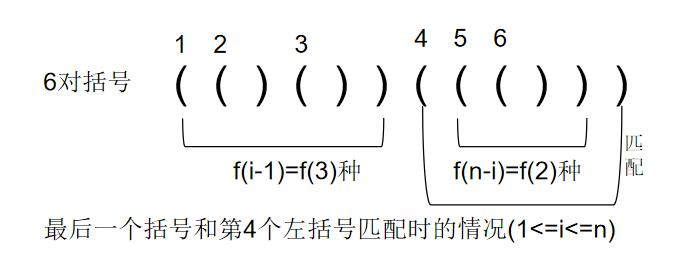
\includegraphics[width=0.7\linewidth]{pic/catalan_proof-001}
	% 	\caption{catalan number - proof}
	% 	\label{fig:catalanproof-001}
	% \end{figure}
	
	
%	\[
%???	(n-3)C_n = \frac{n}{2}(C_3 C_{n-1} + C_4 C_{n-2} + \dots + C_{n-2} C_4 + C_{n-1} C_3 )
%	\]
	第$ n+1 $项 
	\[C(n) = \frac{C^n_{2n}}{n+1} \]
	\[	C(n) = C_{2n}^n-C_{2n}^{n-1} = \frac{C_{2n}^n}{n+1}	\]
	
	通项公式
	\[ C_1 = 1, C_n = C_{n-1}\frac{4n-2}{n+1} \]
	
	
	Python 实现
	
	
	\begin{lstlisting}[language=Python]
		# 打印前 n 个卡特兰数
		ans, n = 1, 20
		print("1:" + str(ans))
		for i in range(2, n + 1):
		ans = ans * (4 * i - 2) // (i + 1)
		print(str(i) + ":" + str(ans))
	\end{lstlisting}
	
	
	扩展\\
	
	最后留一道比较有意思的卡特兰数问题,欢迎读者留言,提出自己的看法。
	
	8 个高矮不同的人需要排成两队,每队 4 个人。其中,每排都是从低到高排列,且第二排的第 i 个人比第一排中第 i 个人高,则有多少种排队方式。
	
	
	
	\section{20.08.07}
	
	\begin{theorem}
	A-G 不等式\\ 任意n个非负实数$ a_1, a_2, \dots, a_n$ \\
	\begin{equation}
		\frac{a_1 + a_2 + \dots + a_n}{n} \geq \sqrt[n]{a_1\dots a_n}
	\end{equation}
	其中等号成立 $\iff a_1 = a_2 = \dots = a_n$

	\label{thm-1}
	\end{theorem}

	\begin{proof}\label{1}
	数学归纳法\\ $n=1$时结论平凡\\
	$n=2\qquad \frac{a_1+a_2}{2} \geq \sqrt{a_1a_2}$\\
	\[(a_1 - a_2)^2 = a_1^2 - 2 a_1 a_2 + a_2^2 \geq 0 \]
	\[a_1^2 + 2a_1a_2 + a_2^2 \geq 4a_1a_2\]
	\[(a_1+a_2)^2\geq 4a_1a_2\]
	\[\frac{a_1+a_2}{2}\geq \sqrt{a_1a_2}\]
	$n=k$时,假设 $\frac{a_1+\dots+a_k}{k}\geq \sqrt[k]{a_1\dots a_k}$成立\\
	$ n=k+1 $
	\begin{equation}
	\begin{aligned}
		&\frac{a_1+\dots + a_k + a_{k+1}}{k+1}-\frac{a_1+\dots +a_k}{k} \\
		=&\frac{k(a_1+\dots+a_{k+1})-(k+1)(a_1+\dots+a_k)}{k(k+1)}\\
		=&\frac{ka_{k+1}-(a_1+\dots+a_k)}{k(k+1)}\\		
	\end{aligned}
	\end{equation}
	we found 
	\[\frac{a_1+\dots + a_k + a_{k+1}}{k+1} =  \frac{a_1+\dots + a_k}{k} + \frac{ka_{k+1}-(a_1+\dots + a_k)}{k(k+1)} \]
	note \[ A := \frac{a_1+\dots + a_k}{k} , \qquad B:=\frac{ka_{k+1}-(a_1+\dots + a_k)}{k(k+1)}\]
	
	\begin{equation}
		(\frac{a_1+\dots + a_k + a_{k+1}}{k+1})^{k+1}=(A+B)^{k+1}\geq A^{k+1}+(k+1)A^k B
	\end{equation}
	使用二项式展开需要对$ a_i $从小到大重排,而使用Bernoulli不等式则只需要$ A\geq 0, (A+B)\geq 0 $即可
	\begin{equation}
		A^{k+1}+(k+1)A^k B = A^k(A+(k+1)B)
	\end{equation}
	\begin{equation}
		\begin{aligned}
			A^k& =	(\frac{a_1+\dots + a_k + a_{k+1}}{k+1})^{k+1} \geq a_1\dots a_k \quad \text{assume at}(n=k)\\
			A+(k+1)B&= \frac{a_1+\dots + a_k}{k} + \frac{ka_{k+1}-(a_1+\dots + a_k)}{k} = a_{k+1}\\
			\because& (A+B)^{k+1}\geq A^k(A+(k+1)B)\geq a_1 \dots a_k  a_{k+1}\\
			\therefore & 	\frac{a_1+\dots + a_k + a_{k+1}}{k+1} \geq  \sqrt[k+1]{a_1 \dots a_k  a_{k+1}}\\
		\end{aligned}
	\end{equation}
	
	使用二项式展开定理的条件:\\
	在归纳法第二步对$a_1 \dots a_{k+1}  $重编号,使$ a_{k+1} $为其中最大的数(之一)\\
	这使得分解式右边第二项$ \frac{ka_{k+1}-(a_1+\dots+a_k)}{k(k+1)} $ 一定是非负数
	\end{proof}
	
	
	\begin{proof}\label{证明 2}
	Forward and backward (Cauchy, 1897)\\
	Forward Part:\\
	$ n=2 $ 
	\begin{equation}
		\frac{a_1+a_2}{2}\geq \sqrt{a_1a_2}
	\end{equation}
	$ n=4 $ 
	\begin{equation}
		\begin{aligned}
			\frac{a_1+a_2+a_3+a_4}{4}
			&\geq \sqrt{\frac{a_1+a_2}{2}\frac{a_3+a_4}{2}}\\
			&\geq \sqrt{\sqrt{a_1a_2}\sqrt{a_3a_4}}\\
			&\geq \sqrt[4]{a_1a_2a_3a_4}\\
		\end{aligned}
	\end{equation}
	$ n=2^k $ 假设不等式$ \frac{a_1+\dots +a_{2^k}}{2^k}\geq \sqrt[2^k]{a_1\dots a_{2^k}} $成立\\
	$ n=2^{k+1} $
	\begin{equation}
		\begin{aligned}
			\frac{a_1+\dots+a_{2^k}+\dots+a_{2^{k+1}}}{2^{k+1}}
			&\geq \sqrt{\frac{a_1+\dots +a_{2^k}}{2^k}\frac{a_{2^k+1}+\dots +a_{2^{k+1}}}{2^k}}\\
			&\geq \sqrt{\sqrt[2^k]{a_1\dots a_{2^k}}\sqrt[2^k]{a_{2^k+1}\dots a_{2^{k+1}}}}\\
			&\geq \sqrt[2^{k+1}]{a_1\dots a_{2^{k+1}}}
		\end{aligned}
	\end{equation}
	
	Backward Part:
	A-G不等式对某个$ n\geq 2 $成立,则它对$ n-1 $也成立
	\begin{equation}
		\begin{aligned}
			\frac{1}{n-1}\sum_{i=1}^{n-1}a_i 
			&= \frac{1}{n}(\frac{n}{n-1})\sum_{i=1}^{n-1}a_i\\
			&=\frac{1}{n}(\sum_{i=1}^{n-1}a_i+\frac{1}{n-1}\sum_{i=1}^{n-1}a_i)
		\end{aligned}
	\end{equation}
	将$ \frac{1}{n-1}\sum_{i=1}^{n-1}a_i $看作$ a_n $
	\begin{equation}
		\frac{1}{n-1}\sum_{i=1}^{n-1}a_i
		\geq \sqrt[n]{(\prod_{i=1}^{n-1}a_i) (\frac{1}{n-1}\sum_{i=1}^{n-1}a_i)}
	\end{equation}
	
	\begin{equation}	
		(\frac{1}{n-1}\sum_{i=1}^{n-1}a_i)^n
		\geq \prod_{i=1}^{n-1}a_i(\frac{1}{n-1}\sum_{i=1}^{n-1}a_i)
	\end{equation}
	

	\begin{equation}	
		(\frac{1}{n-1}\sum_{i=1}^{n-1}a_i)^{n-1}
		\geq \prod_{i=1}^{n-1}a_i
	\end{equation}


	\begin{equation}		
		\frac{1}{n-1}\sum_{i=1}^{n-1}a_i
		\geq \sqrt[n-1]{\prod_{i=1}^{n-1}a_i}
	\end{equation}


	\begin{equation}
		\frac{1}{n-1}\sum_{i=1}^{n-1}a_i \geq \sqrt[n]{(\prod_{i=1}^{n-1}a_i)(\frac{1}{n-1}\sum_{i=1}^{n-1}a_i)}
	\end{equation}
	
	\begin{equation}
		( \frac{1}{n-1}\sum_{i=1}^{n-1}a_i )^n \geq \prod_{i=1}^{n-1}a_i(\frac{1}{n-1}\sum_{i=1}^{n-1}a_i)
	\end{equation}

	\begin{equation}
		( \frac{1}{n-1}\sum_{i=1}^{n-1}a_i )^{n-1} \geq \prod_{i=1}^{n-1}a_i
	\end{equation}
	
	\begin{equation}
		 \frac{1}{n-1}\sum_{i=1}^{n-1}a_i  \geq \sqrt[n-1]{\prod_{i=1}^{n-1}a_i}
	\end{equation}
	
	\end{proof}
	
	\begin{theorem}
		柯西,施瓦茨不等式\\	
		对$ a_1,\dots,a_n $和$ b_1, \dots ,b_n \in \mathbb{R}$,成立
		\begin{equation}
			|\sum_{i=1}^n a_ib_i|\leq \sqrt{\sum_{i=1}^n a_i^2}\sqrt{\sum_{i=1}^n b_i^2}
		\end{equation}
		\label{1.3.5}
	\end{theorem}
	\begin{proof}
		\[ \sum_{i=1}^n (a_i - \lambda b_i)^2 = \sum_{i=1}^n a_i^2 - 2\lambda \sum_{i=1}^n a_i b_i + \lambda^2 \sum_{i=1}^n b_i^2 \geq 0  \]
		由韦达定理(视$ \lambda $为未知数),原方程无解或只有唯一解
		
		\begin{equation}
			\begin{aligned}
				 \Delta = b^2-4ac \leq 0\\
				 (-2\sum_{i=1}^n a_i b_i)^2-4\sum_{i=1}^na_i^2\sum_{i=1}^nb_i^2\leq 0\\	
				 (\sum_{i=1}^n a_i b_i)^2 \leq \sum_{i=1}^na_i^2\sum_{i=1}^nb_i^2\\
				 \sum_{i=1}^n a_i b_i \leq \sqrt{\sum_{i=1}^na_i^2}\sqrt{\sum_{i=1}^nb_i^2}\\
			 \end{aligned}
		\end{equation}
	\end{proof}

	\section{20.08.11}
\begin{theorem}	定积分第一中值定理\\
	设函数$ f(x),g(x) \in \mathbb{C}[a,b]. $且在$ [a,b] $上不变号,则存在$ \zeta \in  [a,b]$,使得$ \int_{a}^{b}f(x)g(x) = f(\zeta)\int_{a}^bg(x)\text{d}x $
	
\end{theorem}
\begin{proof}
	suppose that $ g(x)\ge 0 $. $ f(x) $ continuous on close set,so we can get the maximum and minimum value of $ f $. We note that m is the minimum value of $f(x), x\in [a,b] $,and M is the maximum value of $ f(x) $, then we have:

	\begin{gather}
		mg(x) \le f(x)g(x) \le Mg(x)\\
		m\int_{a}^{b}g(x)\text{d}x \le \int_{a}^{b}f(x)g(x)\text{d}x\le M\int_{a}^{b}g(x)\text{d}x
	\end{gather}

	note that we don't know$ \int_{a}^{b}g(x)\text{d}x \neq 0$
	
	When $ \int_{a}^{b}g(x)\text{d}x = 0$, then $ g(x) \equiv 0 $, So $ \forall \zeta \in [a,b] $, the theorem works.
	
	When $ \int_{a}^{b}g(x)\text{d}x = 0$, then $ m\le \frac{\int_{a}^{b}f(x)g(x)\text{d}x}{\int_{a}^{b}g(x)\text{d}x} \leq M $
	
	From the Intermediate Value Theorem, $ f(x) \in \mathbb{C}[a, b] \quad m\le f(x) \le M $
	
	\begin{gather}
		\exists \zeta \in [a,b] \quad f(\zeta) = \frac{\int_{a}^{b}f(x)g(x)\text{d}x}{\int_{a}^{b}f(x)\text{d}x}\\
		\int_{a}^{b}f(x)g(x)\text{d}x = f(\zeta)\int_{a}^{b}g(x)\text{d}x
	\end{gather}

\end{proof}

设$ g(x) $在$ [a,b] $上连续可积,$ f(x) $在$ [a,b] $上连续单调递增,且$ f'(x) \ge 0 $,并对$ \forall x\in [a,b] $ 有$ f(x)\ge 0 $。则存在$ \zeta \in [a,b] $,使得
\begin{gather}
	\int_{a}^{b}f(x)g(x)\text{d}x = f(b)\int_{\zeta}^{b}g(x)\text{d}x
\end{gather}

\begin{proof}
	set$ G(x) = \int_{x}^{b}g(t)\text{d}t , g(x)\text{在}[a,b] $	上可积

	则$ G(x),x\in [a,b] $存在最值,设最小值和最大值分别为$ m,M $
	
	\begin{gather}
		G(x) = -\int_{b}^{x}g(t)\text{d}t,\quad  G'(x) = -g(x)
	\end{gather}

\begin{equation}
	\begin{aligned}
		\int_{a}^{b}f(x)g(x)\text{d}x &= -\int_{a}^{b}f(x)\text{d}G(x)\\
		&=-{(f(b)G(b) - f(a)G(a)) -\int_{a}^{b}G(x)f'(x)\text{d}x }\\
		&= f(a)G(a)+ \int_{a}^{b}G(x)f'(x)\text{d}x\\
	\end{aligned}
\end{equation}
	\begin{gather}
		m\int_{a}^{b}f'(x)\text{d}x \le \int_{a}^{b} G(x)f'(x)\text{d}x \le M\int_{a}^{b}f'(x)\text{d}x\\
		m[f(b-f(a))] \le  \int_{a}^{b} G(x)f'(x)\text{d}x \le M[f(b-f(a))]\\
	\end{gather}
$ \because $
	\begin{gather}
		mf(a) \le  f(a)G(a) \le Mf(a)\\	
		mf(b) \le  \int_{a}^{b} f(x)g(x) \text{d}x \le Mf(b)\\	
	\end{gather}
% \begin{equation}
% 	\begin{gather}
% 		\text{when} f(b)=0,    &f(x)\equiv 0, \forall \zeta \in [a,b], \text{等式恒成立}\\
% 		\text{when} f(b)\neq0, &m\le \frac{\int_{a}^{b}f(x)g(x)\text{d}x}{f(b)}\le M\\
% 	\end{gather}
% \end{equation}
	From the Intermediate Value Theorem, $ \exists \zeta \in [a,b] s.t. G(\zeta) = \frac{\int_{a}^{b}f(x)g(x)\text{d}x}{f(b)} $\\
	then we have
	\begin{gather}
		\int_{a}^{b}f(x)g(x)\text{d}x = f(b)G(\zeta) = f(b)\int_{\zeta}^{b}g(x)\text{d}x
	\end{gather}
	
	
\end{proof}



	\section{20.08.12}
	1.3.2 练习题
	
	1. 关于Bernoulli不等式的推广:
	\\(1) 证明:当$ -2\ge h\ge -1 $时Bernoulli不等式$ (1+h)^n \ge 1+nh $仍成立;\\
	(2) 证明:当$ h\ge 0 $时成立不等式 
	\begin{equation}
		(1+h)^n\ge \frac{n(n-1)h^2}{2}
	\end{equation} 
	(3) 证明:若$ a_i>-1 \quad (i=1,2,\dots,n) $且同号,则成立不等式\\
	solve:\\
	(1)
	\[ -2 \leq h \leq -1 \]
	\[ -1 \leq 1+h \leq 0 \]
	\[ -1 \leq (1+h)^n \leq 0 \]
	\[ -2n \leq nh \leq -n \]
	\[ 1-2n \leq 1+nh \leq 1-n \]
	
	$ n=0 \qquad (1+h)^0 = 1 = 1+0*h $  结果是平凡的
	
	$ n=1 \qquad 1+h = 1+h $ 结果是平凡的
	
	$ n \geq 2 \qquad $ 此时 $ 1-n \leq -2 $
	\[ 0 \geq (1+h)^n \geq -1 \geq -2 \geq 1-n \geq 1-nh \geq 1- 2n  \]
	\[ (1+h)^n \geq 1+nh \]
	\\
	(2) 
	\[ h\geq 0 \qquad (1+h)^n \geq \frac{n(n-1)h^2}{2} \]
	\[ (1+h)^n=1+nh+\frac{n(n-1)}{2}h^2 + \dots \geq \frac{n(n-1)}{2}h^2  \]
	
	推广:
	\[ (1+h)^n \geq C_n^3 h^3, C_n^4 h^4, \dots , C_n^k h^k ,\qquad 0\leq k\leq n\]
	\\
	(3) 
	\[ \prod_{i=1}^n (1+a_i)\ge 1+\sum_{i=1}^n a_i \]
	(a)$ a_i \ge 0$, 且同号。 
	\[ \prod_{i=1}^n (1+a_i) = 1+ \sum_{i=1}^n a_i + \sum_{i=1,i\neq j}^n \sum_{j=1}^n a_i a_j + \sum_{i=1,i\neq j,k}^n \sum_{j=1,j\neq k}^n \sum_{k=1}^n a_i a_j a_k+\dots \]
	\[ \prod_{i=1}^n (1+a_i) \geq \frac{\prod_{i=1}^n(1+a_i)}{1+a_k} \qquad \forall k\in 1,2,\dots , n,\quad 1+a_k \geq 1 \]
	\\
	(b) $ 0 > a_i > -1 \text{此时} 1 > 1+a_i > 0$
%	\[ \prod_{i=1}^n(1+a_i) \in (0, 1) \]
%	\[ 0> \sum_{i=1}^n a_i >-n \qquad 1>1+\sum_{i=1}^n  a_i >1-n\]
%	\[\text{记}b_i := 1+a_i\qquad a_i = b_i -1, 0<b_i<1\]
%	\[ \prod_{i=1}^n(1+a_i) = \prod_{i=1}^nb_i \]
%	\[1+\sum_{i=1}^na_i = 1+\sum_{i=1}^n(b_i-1)=\sum_{i=1}^n b_i-(n-1)\]
%	$ b_i \in(0,1) $,由A-G不等式
%	\[\frac{1}{n}\sum_{i=1}^n b_i \ge \sqrt[n]{\prod_{i=1}^n b_i}\]
%	\[ \frac{1}{2n-1}[\sum_{i=1}^n b_i - (n-1)] \ge \sqrt[2n-1]{\prod_{i=1}^n b_i\cdot 1^{n-1}} \]
%	\[ \frac{1}{2n-1}[\sum_{i=1}^n a_i + 1] \ge \sqrt[2n-1]{\prod_{i=1}^n (a_i + 1)\cdot 1^{n-1}} \]
	\\别人的方法:
	$ n=1 $时不等式变成等式,显然成立\\
	设$ n=k $时不等式也成立
	\[ \prod_{i=1}^k(1+a_i)\ge 1+\sum_{i=1}^k a_i\]
	则$ n=k+1 $时,有
	\[ \prod_{i=1}^{k+1}(1+a_i) = \prod_{i=1}^k a_i (1 + a_{k+1}) \ge (1+\sum_{i=1}^k a_i) (1+a_{k+1})\]
	\[(1+\sum_{i=1}^k a_i) (1+a_{k+1})=1+\sum_{i=1}^k a_i + a_{k+1} + \sum_{i=1}^k a_i\cdot a_{k+1} \ge 1+\sum_{i=1}^{k+1} a_i \]
	\[\therefore \prod_{i=1}^{k+1}(1+a_i)\ge 1+\sum_{i=1}^{k+1} a_i\]
	
	
	2. 利用A-G不等式求解下列有关阶乘$ n! $的不等式\\
	(1)证明:当$ n>1 $时成立
	\begin{equation}
		n!<(\frac{n+1}{2})^n 
	\end{equation}
	(2)利用$ (n!)^2 = (n\cdot 1)((n-1)\cdot 2)\dots(1\cdot n) $证明:当$ n>1 $时成立
	\begin{equation}
		n!<(\frac{n+2}{\sqrt{6}})^n
	\end{equation}
	(3)比较(1)(2)两个不等式的优劣,并说明原因;\\
	(4)证明:对任意实数$ r $成立
	\begin{equation}
		(\sum_{k=1}^n k^r)^n \ge n^n(n!)^r
	\end{equation}
	solve:\\
	(1) when $ n>1 $
	\[  n! = 1\times 2\times\dots\times n < (\frac{1+2+\dots + n}{n})^n  \]
	\[ (\frac{1+2+\dots + n}{n})^n = (\frac{n(n+1)}{2n})^n = (\frac{n+1}{2})^n \]
	(2) when $ n>1 $
	\[ (n!)^2 = (n\cdot 1)((n-1)\cdot 2)\dots(1\cdot n) < (\frac{n\cdot 1 + (n-1)\cdot 2 + \dots + 1\cdot n}{n})^n \]
	\begin{equation}
		\begin{aligned}
			n\cdot 1 + (n-1)\cdot 2 + \dots + 1\cdot n &= \sum_{k=1}^n (n-k+1)k \\
			\sum_{k=1}^n (n-k+1)k 
			&= (n+1)\sum_{k=1}^n k-\sum_{k=1}^n k^2\\
			&= (n+1)\frac{n(n+1)}{2}-\frac{n(2n+1)(n+1)}{6}\\
			&= \frac{n(n+1)}{6}(3(n+1)-(2n+1))\\
			&= \frac{n(n+1)(n+2)}{6}
		\end{aligned}
	\end{equation}
	
	\begin{equation}
		\begin{aligned}
			(n!)^2  &= (n\cdot 1)((n-1)\cdot 2)\dots(1\cdot n)\\
					&< (\frac{n\cdot 1 + (n-1)\cdot 2 + \dots + 1\cdot n}{n})^n\\
					&= (\frac{1}{n}\frac{n(n+1)(n+2)}{6})^n\\
					&= (\frac{(n+1)(n+2)}{6})^n\\
					&< (\frac{n+2}{6})^{2n}
		\end{aligned}
	\end{equation}

	\begin{equation}
		\therefore \qquad	n! < (\frac{n+2}{\sqrt{6}})^{n}
	\end{equation}
	
	(3) 
	\begin{equation}
		\frac{n+1}{2} = \frac{n+2}{\sqrt{6}}
	\end{equation}
	解得$ n=1+\sqrt{6} >3 $, 
	$ n>3 $时 (2)式更精确,结果比(1)式更好。
	
	(4) $ \forall r \in \mathbb{R} \quad (n!)^r \le \frac{1}{n^n}(\sum_{k=1}^n k^r)^n$
	由A-G不等式
	\begin{equation}
		\frac{1}{n}\sum_{k=1}^n k^r \ge \sqrt[n]{\prod_{k=1}^n k^r}
	\end{equation}
	\begin{equation}
		\begin{aligned}
			(n!)^r  = \prod_{k=1}^n k^r\le (\frac{1}{n}\sum_{k=1}^n k^r)^n =\frac{1}{n^n}(\sum_{k=1}^n k^r)^n
		\end{aligned}
	\end{equation}
	
	\section{20.08.13}
	2.(4) 
	\begin{equation}
		\begin{aligned}
			\forall r \in \mathbb{R} \qquad (\sum_{i=1}^n k^r)^n \ge n^n(n!)^r \\
			 (n!)^r = \prod_{k=1}^n k^r \le (\frac{1^r+2^r+\dots + n^r}{n})^n = \frac{1}{n^n}(\sum_{k=1}^n k^r)^n \quad \text{A-G inequality} \\
			 \therefore (\sum_{k=1}^n k^r)^n \ge n^n(n!)^r\\
		\end{aligned}
	\end{equation}
	
	3. $ a_k >0, \quad k=1,2,\dots, n $ 证明几何-调和平均值不等式
	\begin{equation}
		(\prod_{k=1}^n a_k)^{\frac{1}{n}}\ge \frac{n}{\sum_{k=1}^n\frac{1}{a_k}}
	\end{equation}	
	\begin{proof}
		from A-G inequality 
		\begin{equation}
			\begin{aligned}
				\frac{\sum_{k=1}^n\frac{1}{a_k}}{n} &\ge \sqrt[n]{\prod_{k=1}^n \frac{1}{a_k}} \\
				& =  \frac{1}{\sqrt[n]{\prod_{k=1}^n{a_k}}}\\
				\therefore a_k>0, \qquad {\sqrt[n]{\prod_{k=1}^n{a_k}}}&\ge \frac{n}{\sum_{k=1}^n\frac{1}{a_k}}
			\end{aligned}
		\end{equation}
		
	\end{proof}
	
	
	4. $ a,b,c \ge 0 $, proof that
	\begin{equation}
		\sqrt[3]{abc}\le \sqrt{\frac{ab+bc+ca}{3}}\le\frac{a+b+c}{3}
	\end{equation}
	并推广到n个非负数的情况
	\begin{proof}
		\text{left:}\\
		\begin{equation}
			\begin{aligned}
				\sqrt[3]{abc} &=\sqrt{\sqrt[3]{ab\cdot bc\cdot ca}}\\
				&\le \sqrt{\frac{ab+bc+ca}{3}}
			\end{aligned}
		\end{equation}
		\text{right:}
		\begin{equation}
			\begin{aligned}
				\sqrt{\frac{ab+bc+ca}{3}} &\le \sqrt{\frac{
						(\frac{a+b}{2})^2+
						(\frac{b+c}{2})^2+
						(\frac{c+a}{2})^2
					}{3}}\\
				&=\sqrt{\frac{2(a^2+b^2+c^2)+2(ab+bc+ca)}{12}}\\
				&=\sqrt{\frac{a^2+b^2+c^2+ab+bc+ca}{6}}\\				
			\end{aligned}
		\end{equation}
	
	\begin{equation}
		\because a,b,c \ge 0 \qquad 	\frac{ab+bc+ca}{3} \le \frac{a^2+b^2+c^2+ab+bc+ca}{6}
	\end{equation}
	需要证明 $ \sqrt{\frac{ab+bc+ca}{3}}\le\frac{a+b+c}{3} $\\
	对该式两边平方
	\begin{equation}
		{\frac{ab+bc+ca}{3}}\le\frac{(a+b+c)^2}{9} = \frac{a^2+b^2+c^2 + 2ab+2bc+2ca}{9}
	\end{equation}
	
	\begin{equation}
		\begin{aligned}
			\frac{ab+bc+ca}{3}  &\le \frac{a^2+b^2+c^2}{6} + \frac{ab+bc+ca}{6}\\
								&\le \frac{a^2+b^2+c^2}{6} + \frac{ab+bc+ca}{3}\\
								&= (\frac{a+b+c}{3})^2 \\
			\therefore 	\sqrt{\frac{ab+bc+ca}{3}}  &\le  \frac{a+b+c}{3}\\
		\end{aligned}
	\end{equation}

	\end{proof}
	
	\begin{proof}
		\text{推广至n个}
		\begin{equation}
			\begin{aligned}[l]
				n=2\qquad & \sqrt{ab}      &\le& \frac{a+b}{2} & & \\
				n=3\qquad & \sqrt[3]{abc}  &\le& \sqrt{\frac{ab+bc+ca}{3}}   &\le& \frac{a+b+c}{3}\\
%				n=4\qquad & \sqrt[4]{abcd} &\le \sqrt[3]{\frac{abc+bcd+cda+dab}{4}}    
%				&\le \sqrt{\frac{ab+bc+cd+da}{4}}  &\le \frac{a+b+c+d}{4}  \\
				n=k\qquad & \sqrt[k]{\prod_{i=1}^k a_i}       &\le& \sqrt{\frac{\sum_{i=1}^k-1a_ia_{i+1} + a_ka_1}{k}} &\le& \frac{\sum_{i=1}^ka_i}{k} &\\
			\end{aligned}
		\end{equation}
		
		\begin{equation}
			\text{1} \qquad
			\sqrt[k]{a_1a_2\dots a_k} = \sqrt{\sqrt[k]{a_1^2a_2^2\dots a_k^2}}\le\sqrt{\frac{a_1a_2+a_2a_3+\dots a_ka_1}{k}}
		\end{equation}
		
		\begin{equation}
			\text{2} \qquad
			\sqrt{\frac{a_1a_2+a_2a_3+\dots a_ka_1}{k}} \le \frac{a_1+\dots + a_k}{k}
		\end{equation}
		
		\begin{equation}
			\begin{aligned}
				\frac{a_1a_2+a_2a_3+\dots a_ka_1}{k} &\le \frac{a_1^2 + \dots a_k^2}{2k}\\
				2\frac{a_1a_2+a_2a_3+\dots a_ka_1}{k} &\le \frac{(a_1 + \dots a_k)^2}{2k}\\
				\sqrt{\frac{a_1\dots a_k}{k}} &\le \frac{a_1+\dots +a_k}{\sqrt{4k}}\quad\text{wrong!}
			\end{aligned}
		\end{equation}
		
		
		
	\end{proof}
	
\end{document}
	\chapter{第一章}
\section{引论}
\subsection{关于习题课教案的组织}
\subsection{书中常用记号}
\begin{enumerate}
	\item $ \mathbf{N}_{+} $:所有正整数组成的集合.
	\item $ \mathbf{R} $:所有实数组成的集合(同时也用于表示无限区间$( -\infty,\infty )$).
	\item $ \mathbf{Q} $:所有有理数组成的集合.
	\item $ \mathbf{C} $:所有复数组成的集合.
	\item $ \iff $是等价关系的记号.$ A\iff B $ 表示$ A $和$ B $等价. 例如,$ A $代表$ x > 3 $,$ B $代表$ x-3>0 $,则$ x>3\iff x-3>0 $.
	\item $ [x] $是实数$ x $的整数部分,即不超过$ x $的最大整数. 例如,$ [\sqrt{2}] = 1, [-\sqrt{2}] = -2 $. 关于$ [x] $的基本不等式是:$ [x]\leqslant x < [x] + 1 $,或$ x-1<[x]\leqslant x $
	\item $ \square $表示一个证明或解的结束.
	\item $ {n \choose k} = C_n^k = \frac{n(n-1)\cdots(n-k+1)}{k!}$.
	\item 记号$ \approx $表示近似值. 例如$ \sqrt{2}\approx 1.4 $.
	\item 复合函数$ f(g(x)) $也写成$ (f\circ g)(x) $或$ f \circ g $.
	\item 若$ A $和$ B $为两个集合,则用记号 $ A-B $ 或 $ A \backslash B $ 表示$ A $与$ B $的差集,也就是集合$ \{x|x\in A \text{且} x\notin B\} $.
	\item 用 $ O_\delta (a) $ 表示以$ a $为中心,以$ \delta >0 $ 为半径的邻域. 它就是开区间$ (a-\delta, a+\delta) $(也可以用$ U_\delta (a) $等记号). 如不必指出半径,则可简记为$ O(a)$ (或$ U(a) $).
\end{enumerate}


\subsection{几个常用的初等不等式}
\subsubsection{几个初等不等式的证明}
\begin{theorem}
{1. AG不等式}
n个非负实数 $ a_1,a_2,\cdots,a_n $ 
\begin{equation}
	\frac{a_1+a_2+\cdots+a_n}{n} \ge \sqrt[n]{a_1\cdots a_n}
\end{equation}
$\ge \text{in inequation became} = \iff a_1=a_2=\cdots=a_n$
\end{theorem}

\begin{proof}
	
	method 1. induction method

\begin{align*}
	&k=1 \qquad a_1 = a_1 \\
	&k=2 \qquad \frac{a_1+a_2}{2}\ge\sqrt{a_1a_2} \\	
	&k=n  \qquad \text{suppose }\quad \frac{a_1+a_2+\cdots+a_n}{n} \ge \sqrt[n]{a_1\cdots a_n}  \\
	&k = n+1\\ 	&\qquad\frac{a_1+a_2+\cdots+a_{n+1}}{n+1} - \frac{a_1+a_2+\cdots+a_{n}}{n} \\
	&\qquad=\frac{n(a_1+a_2+\cdots+a_{n+1})-(n+1)(a_1+a_2+\cdots+a_n)}{n(n+1)} \\
	&\qquad=\frac{na_{n+1}-(a_1+a_2+\cdots+a_n)}{n(n+1)}  \\
\end{align*}




Set $ A = \frac{a_1+a_2+\cdots+a_n}{n} $, $ B = \frac{na_{n+1} - (a_1+a_2\cdots+a_n)}{n(n+1)} $\\
\begin{equation*}
	(\frac{a_1+a_2+\cdots+a_{n+1}}{n+1})^{n+1} = (A+B)^{n+1}
\end{equation*}
$ A>0, B\ge 0$
\begin{align*}
	&(A+B)^{n+1} \ge A^{n+1}+(n+1)A^n B\\
	&A^{n+1} + (n+1)A^n B = A^n(A+(n+1)B)\\	
	&A^n = (\frac{a_1+a_2+\cdots+a_n}{n})^n \ge a_1a_2\cdots a_n\\
	&A + (n+1)B = \frac{a_1+a_2+\cdots+a_n}{n} + \frac{na_{n+1}-(a_1+a_2+\cdots+a_n)}{n} = a_{n+1}\\
	&\therefore (A+B)^{n+1} \ge A^n(A+(n+1)B)\ge a_1a_2\cdots a_n\cdot a_{n+1}\\
	&\therefore \frac{a_1+a_2+\cdots+a_{n+1}}{n+1} \ge \sqrt[n+1]{a_1a_2\cdots a_na_{n+1}}\\
\end{align*}

\textbf{使用二项式展开定理的条件}

在归纳法第二步,将$ a_1,a_2,\cdots,a_{n+1} $重编号,使得$ {n+1} $为其中最大的数(之一),这使得分解式右边第二项$ (na_{n+1}-(a_1+a_2+\cdots+a_n))/n(n+1) $一定是非负数。

method 2. Forward and Backward (Cauchy, 1897)

Forward part
\begin{align*}
	&k = 2. \frac{a_1+a_2}{2}\ge \sqrt{a_1a_2}.\\
	&k = 4. \frac{a_1+a_2+a_3+a_4}{4} \ge\sqrt{(\frac{a_1+a_2}{2})\cdot(\frac{a_3+a_4}{2})}.\\
	&\qquad  \ge \sqrt{\sqrt{a_1a_2}\sqrt{a_3a_4}} = \sqrt[4]{a_1a_2a_3a_4}.\\
	&k = 2^n. \text{Suppose}\quad \frac{a_1+a_2+\cdots a_{2^n}}{2^n} \ge \sqrt[2^n]{a_1a_2\cdots a_{2^n}}\\
	&k = 2^{n+1}.\\
	&	\frac{a_1+a_2+\cdots+a_{2^n}+\cdots+a_{2^{n+1}}}{2^{n+1}} \ge \sqrt{(\frac{a_1+a_2+\cdots+a_2^{n}}{2^n})\cdot(\frac{a_{2^{n} + 1}+a_{2^{n}+2}+\cdots+a_2^{n+1}}{2^n})}\\
	&I\ge \sqrt{\sqrt[2^n]{a_1a_2\cdots a_{2^n}}\sqrt[2^n]{a_{2^n+1} a_{2^n+2}\cdots a_{2^{n+1}}}} = \sqrt[2^{n+1}]{a_1a_2\cdots a_{2^{n+1}}}\\
\end{align*}

Backward part
suppose A.G inequality is valid when $ k = n $, Consider $ k = n-1 $.
\begin{align*}
	&\frac{1}{n-1}\sum_{i=1}^{n-1} a_i = \frac{1}{n}(\frac{n}{n-1})\sum_{i=1}^{n-1}a_i\\
	&\frac{1}{n-1}\sum_{i=1}^{n-1} a_i = \frac{1}{n}(\sum_{i=1}^{n-1} a_i + \frac{1}{n-1} \sum_{i=1}^{n-1} a_i)\\
	&\frac{1}{n-1} \sum_{i=1}^{n-1} a_i \ge \sqrt[n]{(\prod_{i=1}^{n-1} a_i)(\frac{1}{n-1}\sum_{i=1}^{n-1} a_i)}\\
	&(\frac{1}{n-1} \sum_{i=1}^{n-1} a_i)^n \ge (\prod_{i=1}^{n-1} a_i)(\frac{1}{n-1}\sum_{i=1}^{n-1} a_i)\\
	&(\frac{1}{n-1} \sum_{i=1}^{n-1} a_i)^{n-1} \ge (\prod_{i=1}^{n-1} a_i)\\
	&\frac{1}{n-1} \sum_{i=1}^{n-1} a_i \ge \sqrt[n-1]{\prod_{i=1}^{n-1} a_i}
\end{align*}
\end{proof}

\begin{proposition}
	{1.3.5 柯西-施瓦茨不等式}
	对$ a_1,a_2,\cdots,a_n $ 和 $ b_1,b_2,\cdots,b_n $,成立
\end{proposition}


\begin{equation*}
	|\sum_{i=1}^n a_i b_i \leqslant \sqrt{\sum_{i=1}^n a_i^2}\sqrt{\sum_{i=1}^n b_i^2}|
\end{equation*}

\begin{proof}
	\begin{equation*}
		 0 \leqslant \sum_{i=1}^n (a_i - \lambda b_i)^2  = \sum_{i=1}^n a_i^2 - 2 \lambda \sum_{i=1}^n a_i b_i  + \lambda^2 \sum_{i=1}^n b_i^2
	\end{equation*}
	由韦达定理 (视$ \lambda $为未知数). 原方程无解或只有唯一解。
	\begin{align*}
		&\Delta = b^2-4ac \leqslant 0\\
		&(-2\sum_{i=1}^n a_i b_i)^2 - 4\sum_{i=1}^n a_i^2 \sum_{i=1}^n b_i^2 \leqslant 0 \\
		&(\sum_{i=1}^n a_i b_i)^2 \leqslant \sum_{i=1}^n a_i^2 \sum_{i=1}^n b_i^2 \\
		&\sum_{i=1}^n a_i b_i \leqslant \sqrt{\sum_{i=1}^n a_i^2} \sqrt{\sum_{i=1}^n b_i^2} 
	\end{align*}
\end{proof}

\subsubsection{练习题}
\begin{example}	关于 Bernoulli 不等式的推广:\\	
	(1) 证明: 当 $ -2 \leqslant h \leqslant -1 $ 时 Bernoulli 不等式 $ (1+h)^n \ge 1+nh $ 仍成立;\\
	(2) 证明: 当 $ h \ge 0 $ 时成立不等式 $ (1+h)^n \ge \frac{n(n-1)h^2}{2} $, 并推广之;\\
	(3) 证明: 若$ a_i > -1(i = 1,2,\dots,n) $ 且同号,则成立不等式
	\[\prod_{i=1}^{n}(1+a_i) \ge 1 + \sum_{i=1}^n a_i \]
	\begin{proof}
		(1)			
		\begin{align*}
			& -2 \leqslant h \leqslant -1  & \\
			& -1 \leqslant 1+h\leqslant 0  & -1 \leqslant (1+h)^n \leqslant 0 \\
			& -2n \leqslant nh \leqslant -n& 1-2n \leqslant 1+nh\leqslant 1-n
		\end{align*}	
		\begin{align*}
			n=0. && (1+h)^0 = 1 = 1 + 0\times h\\
			n=1. && 1+h = 1+h\\
			n \ge 2. && 1-n \leqslant -2
		\end{align*}	
		\begin{align*}
			0 \ge (1+h)^n \ge -1 \ge -2 \ge 1-n \ge 1+nh \ge 1-2n
		\end{align*}	
		\begin{align*}		
			(1+h)^n \ge 1+nh
	 	\end{align*}
	
		(2)
		\begin{align*}
			h\ge 0&\\
			(1+h)^n = &1+nh+\frac{n(n-1)}{2}h^2 + \dots \ge \frac{n(n-1)}{2}h^2\\
		\end{align*}
		推广:
		\begin{equation*}
			(1+h)^n \ge \binom{n}{3}h^3, \binom{n}{4}h^4, \dots, \binom{n}{k}h^k, 0\leqslant k \leqslant n
		\end{equation*}
		
		(3)
%		\begin{align*}
%			\prod_{i=1}^n(1+a_i) = 1+\sum_{i=1}^n a_i + \sum_{i=1}^n\sum_{j=1}^n a_i a_j + 	\sum_{i=1}^n\sum_{j=1}^n\sum_{k=1}^n a_i a_j a_k + \dots
%		\end{align*}
%		分类讨论\\
%		1. $ a_i\ge 0, 1+a_i \ge 1 $. 
%		\[ \prod_{i=1}^n (1+a_i) \ge \frac{\prod_{i=1}^n (1+a_i)}{1+a_k} \qquad\forall k \in 1,2, \dots,n \]
		$ k = 1 $ 时显然成立. 使用归纳法证明. 假设$ k = n $ 时不等式
		$ \prod_{i=1}^{n}(1+a_i) \ge 1 + \sum_{i=1}^n a_i  $
		成立, 证明 $ k = n+1 $时 
		$  \prod_{i=1}^{n+1}(1+a_i) \ge 1 + \sum_{i=1}^{n+1} a_i  $
		成立.		
		\begin{align*}
			k = n+1 \qquad  
			& \prod_{i=1}^{n+1}(1+a_i) = \prod_{i=1}^{n}(1+a_i)  (1+a_{n+1})\\
			& \because \prod_{i=1}^{n}(1+a_i) \ge 1 + \sum_{i=1}^n a_i  \\
			& \prod_{i=1}^{n}(1+a_i)  (1+a_{n+1}) \ge (1 + \sum_{i=1}^n a_i)(1+a_{n+1})
		\end{align*}
		\begin{align*}
			(1 + \sum_{i=1}^n a_i)(1+a_{n+1}) & = 1 + \sum_{i=1}^n a_i + a_{n+1} + a_{n+1} \sum_{i=1}^n a_i\\
			& = 1 + \sum_{i=1}^{n+1} a_i + a_{n+1} \sum_{i=1}^n a_i\\
			& \ge 1 + \sum_{i=1}^{n+1} a_i
		\end{align*}
	\end{proof}
\end{example}

\begin{example}
	利用 A.G.不等式求解:\\
	(1). $ n! \leqslant (\frac{n+1}{2})^n, \text{while } n >1 $\\
	(2). $ (n!)^2 = (n\cdot 1)[(n-1)\cdot 2]\dots (1\cdots n) $. 证明: 当$ n > 1 $时成立
	\[n!< (\frac{n+2}{6})^n\]
	(3). 比较上述两个不等式的优劣\\
	(4). 证明: 对任意实数r成立:
	\begin{equation}\label{FactorialNPowerR}
		(n!)^r\leqslant  \frac{1}{n^n} (\sum_{k=1}^n k^r)^n 
	\end{equation}
	\begin{proof}
		(1).
		\begin{align*}
			n>1 \qquad & n! = 1 \times 2 \times \cdots \times n < (\frac{1+2+\cdots + n}{n})^n = (\frac{(1+n)n}{2n})^n = (\frac{n+1}{2})^n
		\end{align*}
		$ \because 1 \neq 2 \neq \cdots n $, 所以不会有等号出现的情况\\
		(2). $ n > 1 $
		\begin{align*}		
			 (n!)^2 
			 & = (n\cdot 1)[(n-1)\cdot 2]\dots (1\cdots n)\\
			 & < (\frac{n\times1 + (n-1)\times 2 + \dots + 1\times n}{n})^n\\
		\end{align*}
		Consider this equation 
		\begin{equation}\label{keyn1nminus12}
			 (\frac{n\times1 + (n-1)\times 2 + \dots + 1\times n}{n})^n 
		\end{equation}
		\begin{align*}
			\sum_{k=1}^n (n-k+1)k 
			& = (n+1)\sum_{k=1}^nk - \sum_{k=1} k^2\\
			& = (n+1)\frac{(n+1)n}{2} - \frac{n(n+1)(2n+1)}{6}\\	
			& = \frac{n(n+1)}{6}(3(n+1) - (2n+1))\\
			& = \frac{n(n+1)(n+2)}{6}
		\end{align*}
		\begin{align*}		
			(n!)^2 
			& <  (\frac{n\times1 + (n-1)\times 2 + \dots + 1\times n}{n})^n\\
			& = (\frac{(n+1)(n+2)}{6})^n
		\end{align*}
		$ \because n+1<n+2 $,
		$ \therefore n! < (\frac{n+2}{\sqrt{6}})^n $\\
		(3). $ n>3 $时,$ \frac{n+2}{\sqrt{6}} < \frac{n+1}{2} $ (2)的结果较好.\\
		(4). $  \forall r\in \mathbb{R} $, prove formula \ref{FactorialNPowerR}
		\begin{align*}
			&\frac{1}{n}\sum_{k=1}^n k^r \ge \sqrt[n]{\prod_{k=1}^n k^r}\\
			&(n!)^r =\prod_{k=1}^n k^r \leqslant (\frac{1}{n}\sum_{k=1}^n k^r)^n = \frac{1}{n^n}(\sum_{k=1}^n k^r)^n 
		\end{align*}
	my answer
	\begin{align*}
		&\forall r\in \mathbb{R},\qquad(\sum_{k=1}^n k^r)^n \ge n^n(n!)^r\\
		&(n!)^r = \sum_{k=1}^n k^r \leqslant (\frac{1^r+2^r+\dots+n^r}{n})^n = \frac{1}{n^n}(\sum_{k=1}^n k^r)^n\\
		&\therefore\quad (\sum_{k=1}^n k^r)^n \ge n^n(n!)^r
 	\end{align*}
	\end{proof}
\end{example}

\begin{example}
	$ a_k>0, k = 1,2,\dots,n$ 证明几何--调和平均值不等式
	\[(\prod_{k=1}^n a_k)^{\frac{1}{n}} \ge \frac{n}{\sum_{k=1}^n\frac{1}{a_k}}\]
	\begin{proof}
		from A.G inequality
		\[\frac{\sum_{k=1}^n\frac{1}{a_k}}{n} \ge \sqrt[n]{\prod_{k=1}^n \frac{1}{a_k}} = \frac{1}{\sqrt[n]{\prod_{k=1}^n a_k}}\]
		\[a_k>0, \quad \sqrt[n]{\prod_{k=1}^n {a_k}} \ge  \frac{n}{\sum_{k=1}^n\frac{1}{a_k}} \]
	\end{proof}
\end{example}

\begin{example}
	$ a,b,c\ge 0. $ prove $ \sqrt[3]{abc}\le\sqrt{\frac{ab+bc+ca}{3}} \leqslant \frac{a+b+c}{3} $.
	并推广到n个非负数的情况
	\begin{proof}
		1. $ \sqrt[3]{abc} = \sqrt{\sqrt[3]{ab\cdot bc\cdot ca}} \leqslant \sqrt{\frac{ab+bc+ca}{3}} $.\\
		2. 
		\begin{align*}
			\sqrt{\frac{ab+bc+ca}{3}} 
			\leqslant &\sqrt{\frac{(\frac{a+b}{2})^2+(\frac{b+c}{2})^2+(\frac{c+a}{2})^2}{3}} \\
			&= \sqrt{\frac{2(a^2+b^2+c^2)+2(ab+bc+ca)}{12}}\\
			&= \sqrt{\frac{a^2+b^2+c^2+ab+bc+ca}{6}}
		\end{align*}
		$ a,b,c\ge 0 $, 希望证明\[\sqrt{\frac{ab+bc+ca}{3}}\leqslant \frac{a+b+c}{3}\]
		\begin{align*}
			\frac{ab+bc+ca}{3} &\leqslant \frac{a^2+b^2+c^2}{6} + \frac{ab+bc+ca}{6}\\
			\frac{ab+bc+ca}{2} &\leqslant \frac{a^2+b^2+c^2}{6} + 2\frac{ab+bc+ca}{6}\qquad(\text{add} \frac{ab+bc+ca}{6})\\
			\frac{ab+bc+ca}{3} &\leqslant \frac{ab+bc+ca}{2} \leqslant (\frac{a+b+c}{3})^2\\
			&\sqrt{\frac{ab+bc+ca}{3}} \leqslant \frac{a+b+c}{3}
		\end{align*}
		推广至n个
		\begin{align*}[l]
			n=2\qquad& \sqrt{ab} \le\frac{a+b}{2}\\
			n=3\qquad& \sqrt[3]{abc}  \leqslant \sqrt{\frac{ab+bc+ca}{3}} \leqslant \frac{a+b+c}{3}\\
			n=4\qquad& \sqrt[4]{abcd}  \leqslant \sqrt[3]{\frac{abc+bcd+cda+dab}{4}} \leqslant \sqrt{\frac{a+b+c}{3}}\le\frac{a+b+c+d}{4}
		\end{align*}
		\begin{align*}
			k = n \qquad& \sqrt[n]{a_1a_2\dots a_n} \leqslant 		\sqrt{\frac{a_1+a_2+\dots+a_n}{n}}\le\frac{a_1+a_2+\dots+a_n}{n}
		\end{align*}
		This is
		\begin{align*}
			\sqrt[n]{\sum_{k=1}^n a_k} \leqslant \sqrt{\frac{\sum_{k=1}^n a_k}{k}}\le\frac{\sum_{k=1}^n a_k}{k}
		\end{align*}
		1. $ \sqrt[n]{a_1 a_2 \dots a_n} = \sqrt{\sqrt[n]{a_1^2 a_2^2 \dots a_n^2}} \leqslant \sqrt{\frac{a_1 a_2 + a_2 a_3 + \dots + a_n a_1}{n}}$\\
		2. $ \sqrt{\frac{a_1 a_2 + a_2 a_3 + \dots + a_n a_1}{n}} \leqslant \sqrt{\frac{a_1+ a_2 + \dots + a_n}{n}} $?
	\end{proof}
\end{example}

\begin{example}
	(1) $ |\alpha + \beta | \leqslant |\alpha| + |\beta|$
	\begin{proof}
		let $ \alpha = a-b, \beta = b $, the identity became $ |(a-b) + b| \leqslant |a-b| + |b| $. This is $ |a - b| \ge |a| - |b| $.
		\begin{equation*}
			||a| - |b|| = \Big\lbrace %\left\lbrace  \right % empty \right for tex grammer check!
			\begin{aligned}
				|a| - |b|. \qquad a \ge b\\
				|b| - |a|. \qquad a < b
			\end{aligned}
		\end{equation*}
		When $ a\ge b $, $ ||a| - |b|| = |a| - |b| $. There is $ |a-b| \ge |a| - |b| = ||a|-|b|| $\\
		When $ a < b $, $ |a-b| = |b-a| \ge |b| - |a|  = ||a|-|b|| $.\\
		$ \therefore $, We have$ |a-b| \ge ||a|-|b|| $
	\end{proof}
		
	(2) $ \sum |a_k| \ge |\sum a_k|$ 
	\begin{proof}
		We can prove this statement by induction.
		\begin{align*}
			k=2,\qquad&|a_1| + |a_2| \ge |a_1+a_2|\\
			k=3,\qquad&|a_1| + |a_2| + |a_3| \ge |a_1+a_2+a_3|\\
			\text{Suppose } k = n, \qquad & \sum_{k=1}^n |a_k| \ge |\sum_{k=1}^n a_k| \\
			k = n+1, \qquad& \text{prove}\sum_{k=1}^{n+1} |a_k| \ge |\sum_{k=1}^{n+1} a_k|
		\end{align*}
		\begin{align*}
			\sum_{k=1}^{n+1} |a_k| 
			&= \sum_{k=1}^{n} |a_k| + |a_{n+1}| \\
			&\ge |\sum_{k=1}^n a_k| + |a_{n+1}| \\
			&\ge |\sum_{k=1}^{n+1} a_k|
		\end{align*}
	
		\begin{align*}
			k=2,\qquad&|a_1| - |a_2| \leqslant |a_1-a_2|\\
			\text{Suppose } k = n, \qquad & |a_1| - \sum_{k=2}^n |a_k| \leqslant |\sum_{k=1}^n a_k| \\
			k = n+1, \qquad& \text{prove}|a_1| - \sum_{k=2}^{n+1} |a_k| \leqslant |\sum_{k=1}^{n+1} a_k|
		\end{align*}
		\begin{align*}
			|a_1| - \sum_{k=2}^{n+1} |a_k| 
			&= |a_1| - \sum_{k=2}^{n} |a_k| - |a_{n+1}| \\
			&\leqslant |\sum_{k=1}^n a_k| - |a_{n+1}| \\
			&\leqslant |\sum_{k=1}^{n+1} a_k|
		\end{align*}
		Can left side became$ \left| |a_1| - \sum_{k=2}^n|a_k|\right| $?
		\begin{equation}\label{a1ak_eq1}
			\left| |a_1| - \sum_{k=2}^n|a_k|\right| = |a_1| - \sum_{k=2}^n|a_k| \qquad |a_1| \ge\sum_{k=2}^n a_k
		\end{equation}
		\begin{equation}\label{a1ak_eq2}
			\left| |a_1| - \sum_{k=2}^n|a_k|\right| = \sum_{k=2}^n|a_k| - |a_1| \qquad |a_1| \ge\sum_{k=2}^n a_k
		\end{equation}
		in eq\ref{a1ak_eq1}, the inequality is still vaild. However in eq\ref{a1ak_eq2}, $ \sum_{k=2}^n |a_k| - |a_1| $ and $ |a_1| $
	\end{proof}
	(3). $\frac{|a+b|}{1+|a+b|}\leqslant \frac{|a|}{1+|a|} + \frac{|b|}{1+|b|} $
	\begin{proof}
%		\begin{align*}
%			\frac{|a+b|}{1+|a+b|}\leqslant &\frac{|a|}{1+|a|} + \frac{|b|}{1+|b|}\\
%			1-\frac{1}{1+|a+b|}\le&2-(\frac{1}{1+|a|} + \frac{1}{1+|b|})\\
%			& = 2-\frac{2+|a|+|b|}{(1+|a|)(1+|b|)}\\
%			& = 1-\frac{2+|a|+|b|-(1+|a|)(1+|b|)}{(1+|a|)(1+|b|)}\\
%			& = 1-\frac{1-|a||b|}{(1+|a|)(1+|b|)}
%		\end{align*}
	\begin{align*}
		\frac{|a+b|}{1+|a+b|}\leqslant &\frac{|a|}{1+|a|} + \frac{|b|}{1+|b|}\\
		\frac{|a+b|}{1+|a+b|}\leqslant &\frac{|a|+|b|+2|a||b|}{(1+|a|)(1+|b|)}\\
		1-\frac{|a+b|}{1+|a+b|}\ge &1-\frac{|a|+|b|+2|a||b|}{(1+|a|)(1+|b|)}\\
		\frac{1}{1+|a+b|}\ge &\frac{1-|a||b|}{(1+|a|)(1+|b|)}\\
		1+|a|+|b|+|a||b| \ge & 1+|a+b|-|a||b|-|a||b||a+b|\\
		|a|+|b|+2|a||b|+|a||b||a+b|>&0, \text{Since }+2|a||b|+|a||b||a+b|\ge|a+b|
	\end{align*}
	Therefore $\frac{|a+b|}{1+|a+b|}\leqslant \frac{|a|}{1+|a|} + \frac{|b|}{1+|b|} $
	\end{proof}
%	\begin{align*}
%		1-\frac{1}{1+|a+b|}\le
%		&2-(\frac{1}{1+|a|} + \frac{1}{1+|b|})\\
%		& = 2-\frac{2+|a|+|b|}{(1+|a|)(1+|b|)}\\
%		& = 1-\frac{2+|a|+|b|-(1+|a|)(1+|b|)}{(1+|a|)(1+|b|)}\\
%		& = 1-\frac{1-|a||b|}{(1+|a|)(1+|b|)}
%	\end{align*}
%	We only need to prove that $ \frac{1}{1+|a+b|} \ge \frac{1-|a||b|}{(1+|a|)(1+|b|) $. We already know that $ |a||b| = |ab| $.
%		\begin{align*}
%			&(1+|a|)(1+|b|) &\ge (1+|a+b|)(|ab|-1)\\
%			&1+|a|+|b|+|ab| &\ge |ab|+|ab|\cdot|a+b|-1-|a+b|\\
%			&2+|a|+|b|+|a+b| &\ge |ab|\cdot|a+b|\
%		\end{align*}
%		\begin{align*}
%			|a+b|&\le|a|+|b|\\
%			1+|a+b|&\leqslant 1+|a|+|b|\\
%			&\leqslant 1+|a|+|b|+|a||b|\\
%			&=(1+|a|)(1+|b|)
%		\end{align*}
\end{example}

\begin{example}
	(4).$ |(a+b)^n-a^n| \leqslant (|a|+|b|)^n-|a|^n $
	\begin{align*}
		(a+b)^n-a^n &= \binom{n}{1}a^{n-1}b^{1} + \binom{n}{2}a^{n-2}b^{2} + \cdots + \binom{n}{n}a^{0}b^{n}\\
		(|a|+|b|)^n-|a|^n &= \binom{n}{1}|a|^{n-1}|b|^{1} + \binom{n}{2}|a|^{n-2}|b|^{2} + \cdots + \binom{n}{n}|a|^{0}|b|^{n}
	\end{align*}
	\begin{align*}
		&\because |a|^j|b|^k \ge a^j b^k\\
		&\therefore \sum |a|^j|b|^k \ge |\sum a^j b^k|
	\end{align*}
\begin{align*}
	|(a+b)^n-a^n| = \Big\lbrace 
	\begin{aligned}
		(a+b)^n-a^n,\qquad a+b\ge a; b\ge0\\
		a^n-(a+b)^n,\qquad a+b< a; b<0
	\end{aligned}
\end{align*}
\begin{equation}\label{keyEx134answer}
	|(a+b)^n-a^n| \leqslant (|a|+|b|)^n - |a|^n.
\end{equation}
\end{example}

\begin{proposition}
	{1.3.5(Cauchy inequality)}
	For $ a_1,a_2,\dots,a_n.$ and $b_1,b_2,\dots,b_n$. $ a_i,b_i\in\mathbb{R} $, There is
	\begin{equation}\label{CauchyInequality}
		\Big|\sum_{i=1}^n a_i b_i\Big| \leqslant \sqrt{\sum_{i=1}^n a_i^2}\sqrt{\sum_{i=1}^n b_i^2}
	\end{equation}
\end{proposition}
\begin{proof}
	Let's prove eq\ref{CauchyInequality}\\
	First way on book:\\
	Use variable $ \lambda $, change the inequality into nonnegative binomial.
	\begin{align*}
		0&\le\sum_{i=1}^n (a_i -\lambda b_i)^2 
		&=\sum_{i=1}^n a_i^2 - 2\lambda\sum_{i=1}^na_ib_i + \lambda^2\sum_{i=1}^n\\
		\Delta &= B^2-4AC &=(-2\sum_{i=1}^n a_ib_i)^2 - 4(\sum_{i=1}^na_i^2)(\sum_{i=1}^nb_i^2)\le0\\	
	\end{align*}
	\begin{equation*}
		(\sum_{i=1}^n a_ib_i)^2 \leqslant (\sum_{i=1}^na_i^2)(\sum_{i=1}^nb_i^2)
	\end{equation*}
	sqrt on both side of the inequality above, we can get
	\begin{equation*}
		\Big|\sum_{i=1}^n a_i b_i\Big| \leqslant \sqrt{\sum_{i=1}^n a_i^2}\sqrt{\sum_{i=1}^n b_i^2}
	\end{equation*}
\end{proof}
6. Cauchy 不等式的不同证明

(1). 数学归纳法.\\
\begin{align*}
	k=1,\quad& |ab|=\sqrt{a^2}\sqrt{b^2}\\
	k=1,\quad& |a_1b_1+a_2b_2|=\sqrt{a_1^2+a_2^2}\sqrt{b_1^2+b_1^2}\\
	\text{Suppose }k=n,\quad&|\sum_{i=1}^n a_ib_i|=\sqrt{\sum_{i=1}^n a_i}\sqrt{\sum_{i=1}^n b_i}\\
	k=n+1,\quad&|\sum_{i=1}^{n+1} a_ib_i|=|\sum_{i=1}^{n} a_ib_i + a_{n+1}b_{n+1}|
\end{align*}
\begin{align*}
	|\sum_{i=1}^{n+1} a_ib_i|
	&=|\sum_{i=1}^{n} a_ib_i + a_{n+1}b_{n+1}|\\
%	&\le|\sum_{i=1}^{n} a_ib_i| + |a_{n+1}b_{n+1}|\\
	&\le|\sqrt{\sum_{i=1}^n a_i}\sqrt{\sum_{i=1}^n b_i} + a_{n+1}b_{n+1}|\\
\end{align*}
Note that $ A = \sqrt{\sum_{i=1}^n a_i} $, $ B = \sqrt{\sum_{i=1}^n b_i} $
\begin{align*}
	|\sum_{i=1}^{n+1} a_ib_i|
	&\le|AB+a_{n+1}b_{n+1}|\\
	&\le\sqrt{A^2+a_{n+1}^2}\sqrt{B^2+b_{n+1}^2}\\
	&=\sqrt{\sum_{i=1}^na_i^2}\sqrt{\sum_{i=1}^nb_i^2}
\end{align*}
(2) Lagrange 恒等式
\begin{equation}
	\sum_{i=1}^n a_k^2\sum_{i=1}^n b_k^2 - (\sum_{i=1}^n |a_kb_k|) = \frac{1}{2}\sum_{i=1}^n\sum_{k=1}^n(|a_k||b_i|-|a_i||b_k|)^2
\end{equation}
\begin{align*}
	(|a_k||b_i|-|a_i||b_k|)^2 
	&= |a_k|^2|b_i|^2-2|a_i||a_k||b_i||b_k|+|b_k|^2|a_i|^2\\
	&= a_k^2b_i^2+b_k^2a_i^2-2|a_ia_kb_ib_k|
\end{align*}
\begin{equation*}
	\sum_{i=1}^n\sum_{k=1}^n(|a_k||b_i|-|a_i||b_k|)^2 = 2\sum_{i=1}^n a_i^2 \sum_{k=1}^n b_k^2 - 2\sum_{i=1}^n\sum_{k=1}^n|a_ia_kb_ib_k|
\end{equation*}
\begin{equation*}
	\sum_{i=1}^n a_k^2\sum_{i=1}^n b_k^2 - (\sum_{i=1}^n |a_kb_k|) = \frac{1}{2}\sum_{i=1}^n\sum_{k=1}^n(|a_k||b_i|-|a_i||b_k|)^2 \ge 0
\end{equation*}
\begin{align*}
	&\therefore (\sum_{i=1}^n|a_ib_i|)^2 \leqslant \sum_{i=1}^na_i^2 \sum_{i=1}^nb_i^2\\
	&\because |\sum_{i=1}^n a_i b_i| \leqslant \sum_{i=1}^n|a_ib_i|\\
	&\therefore (|\sum_{i=1}^n a_i b_i|)^2 \leqslant (\sum_{i=1}^n|a_ib_i|)^2\\
	&\therefore (|\sum_{i=1}^n a_i b_i|)^2 \leqslant \sum_{i=1}^n a_i^2 \sum_{i=1}^n b_i^2
\end{align*}
不等式两边开平方,得到:
\begin{equation*}
	|\sum_{i=1}^n a_i b_i| \leqslant \sqrt{\sum_{i=1}^n a_i^2} \sqrt{\sum_{i=1}^n b_i^2}
\end{equation*}

(3). 用不等式 $ |AB| \leqslant \frac{A^2+B^2}{2} $
\begin{align*}
	|a_ib_i| &\leqslant \frac{a_i^2+b_i^2}{2}&\\
	|\sum_{i=1}^na_ib_i| &\leqslant \sum_{i=1}^n|a_ib_i|&\leqslant \frac{\sum_{i=1}^n a_i^2+\sum_{i=1}^n b_i^2}{2}\\
	\frac{\sum_{i=1}^na_i^2+\sum_{i=1}^nb_i^2}{2} &\ge \sqrt{\sum_{i=1}^n a_i^2} \sqrt{\sum_{i=1}^n b_i^2} &\text{??}
\end{align*}
如何用均值不等式证明Cauchy不等式?\\
由切比雪夫不等式,有
\begin{equation}\label{CauchyInequality002}
	\frac{a_1b_1+a_2b_2+\cdots+a_nb_n}{n} \leqslant (\frac{a_1+a_2+\cdots+a_n}{n}) (\frac{b_1+b_2+\cdots+b_n}{n})
\end{equation}
由均值不等式,有
\begin{align*}
	\frac{a_1+a_2+\cdots+a_n}{n} &\leqslant \sqrt{\frac{a_1^2+a_2^2+\cdots+a_n^2}{n}}\\
	\frac{b_1+b_2+\cdots+b_n}{n} &\leqslant \sqrt{\frac{b_1^2+b_2^2+\cdots+b_n^2}{n}}
\end{align*}
\begin{align*}
	\therefore \frac{a_1b_1+a_2b_2+\cdots+a_nb_n}{n} 
	&\leqslant (\frac{a_1+a_2+\cdots+a_n}{n}) (\frac{b_1+b_2+\cdots+b_n}{n}) \\
	&\leqslant \sqrt{\frac{a_1^2+a_2^2+\cdots+a_n^2}{n}} \sqrt{\frac{b_1^2+b_2^2+\cdots+b_n^2}{n}}\\
	& = \frac{1}{n}\sqrt{a_1^2+a_2^2+\cdots+a_n^2} \sqrt{b_1^2+b_2^2+\cdots+b_n^2}\\
\end{align*}
This is 
\begin{equation*}
	\sum_{i=1}^n a_i b_i \leqslant \sqrt{\sum_{i=1}^n a_i^2} \sqrt{\sum_{i=1}^n b_i^2}
\end{equation*}
Square on both side of the inequality, The calculate square root. We can get eq\ref{CauchyInequality002}:

(4). 构造复的辅助数列
\begin{equation*}
	c_k = a_k^2 - b_k^2 + 2i |a_k b_k|, \qquad k = 1,2,\dots, n
\end{equation*}
Then we use
\begin{equation*}
	\Big|\sum_{k=1}^n c_k\Big| \leqslant \sum_{k=1}^n |c_k|
\end{equation*}

%\begin{solve}
	\begin{align*}
		&c_k = (|a_k| + i |b_k|)^2 = a_k^2 + b_k^2 + 2i |a_k b_k|\\
		&\sum_{k=1}^n c_k = \sum_{k=1}^n a_k^2 + \sum_{k=1}^n b_k^2 + 2i \sum_{k=1}^n |a_k b_k|\\
		&|c_k| = \sqrt{\Re^2 c_k + \Im^2 c_k} = \sqrt{(a_k^2-b_k^2)^2 + (2a_kb_k)^2} = a_k^2+b_k^2
	\end{align*}
	\begin{align*}
		&\therefore \Big| \sum_{k=1}^n a_k^2 + \sum_{k=1}^n b_k^2 + 2i \sum_{k=1}^n |a_k b_k| \Big|
		= \sqrt{\Re^2 \sum_{k=1}^n c_k + \Im^2 \sum_{k=1}^n c_k}\\
		&= \sqrt{(\sum_{k=1}^n (a_k^2-b_k^2))^2 + \sum_{k=1}^n (2a_kb_k)^2}\\
		&= \sqrt{(\sum_{k=1}^n a_k^2)^2 + (\sum_{k=1}^n a_k^2)^2 - 2(\sum_{k=1}^n a_k^2)(\sum_{k=1}^n a_k^2) + 4\sum_{k=1}^n (a_kb_k)^2}\\	
 		&\because |\sum c_k| \leqslant \sum|c_k| \\
 		&\therefore  (\sum_{k=1}^n a_k^2)^2 + (\sum_{k=1}^n a_k^2)^2 - 2(\sum_{k=1}^n a_k^2)(\sum_{k=1}^n a_k^2) + 4\sum_{k=1}^n (a_kb_k)^2 \leqslant (\sum_{k=1}^n a_k^2 + \sum_{k=1}^n b_k^2)^2\\
 		&\therefore 4(\sum_{k=1}^n a_k b_k)^2 \leqslant 4(\sum_{k=1}^n a_k^2) (\sum_{k=1}^n b_k^2)\\
 		& \text{extracting both side: } \Big|\sum_{k=1}^n a_k b_k\Big| \leqslant \sqrt{\sum_{k=1}^n a_k^2} \sqrt{\sum_{k=1}^n b_k^2}
\end{align*}
%\end{solve}

\begin{example}
	7. Suppose $ 0<x_i\leqslant \frac{1}{2}, i=1,2,\dots,n $, then
	\begin{equation}\label{ex17FormulaByFanKy}
		\frac{\prod_{i=1}^n x_i}{(\sum_{i=1}^n x_i)^n} \leqslant \frac{\prod_{i=1}^n(1-x_i)}{(\sum_{i=1}^n(1-x_i))^n}
	\end{equation}
\begin{proof}
	Let's prove eq\ref{ex17FormulaByFanKy} by induction method.
	\begin{equation*}
		n=2,\qquad \frac{x_1x_2}{(x_1+x_2)^2}\leqslant \frac{(1-x_1)(1-x_2)}{((1-x_1)+(1-x_2))^2}
	\end{equation*}
	\begin{align*}
		&\frac{(x_1x_2)}{(x_1^2+2x_1x_2+x_2^2)} \leqslant \frac{1-x_1-x_2+x_1x_2}{(1-x_1)^2+2(1-x_1)(1-x_2)+(1-x_2)^2}\\
		&\frac{(x_1+x_2)^2}{(x_1x_2)} \ge \frac{((1-x_1)(1-x_2))^2}{1-x_1-x_2+x_1x_2}\\
		&\frac{x_1}{x_2} + 2 + \frac{x_2}{x_1} \ge \frac{1-x_1}{1-x_2} + 2\frac{1-x_2}{1-x_1}\\
		&\frac{x_1}{x_2} - \frac{1-x_1}{1-x_2} \ge \frac{1-x_2}{1-x_1} - \frac{x_2}{x_1}\\
		&\frac{x_1(1-x_2) - x_2(1-x_1)}{x_2(1-x_2)} \ge \frac{x_1(1-x_2)-x_2(1-x_1)}{x_1(1-x_1)}\\
		&\frac{x_1-x_2}{x_2(1-x_2)} \ge \frac{x_1 - x_2}{x_1(1-x_1)}
	\end{align*}
$ f(x) = x-x^2, f'(x) = 1-2x>0,\text{ while }x\in(0,\frac{1}{2})  $\\
When $ x_1>x_2 , 0<x_2<x_1\leqslant \frac{1}{2}, x_1-x_1^2 \ge x_2-x_2^2, x_1-x_2>0$\\
When $ x_1<x_2 , 0<x_1<x_2\leqslant \frac{1}{2}, x_1-x_1^2 \leqslant x_2-x_2^2, x_1-x_2<0$\\
\begin{equation*}
	 \frac{x_1-x_2}{x_2(1-x_2)} \ge \frac{x_1 - x_2}{x_1(1-x_1)} 
\end{equation*}
\begin{align*}
	&k=2,\qquad \frac{x_1x_2}{(x_1+x_2)^2}\leqslant \frac{(1-x_1)(1-x_2)}{((1-x_1)+(1-x_2))^2}\\
	&k=4,\qquad \frac{x_1x_2x_3x_4}{(x_1+x_2+x_3+x_4)^2}\leqslant 
	\frac{(1-x_1)(1-x_2)(1-x_3)(1-x_4)}{((1-x_1)+(1-x_2)+(1-x_3)+(1-x_4))^2}\\
	&\text{Use Cauchy's forward and backward method, We can prove this equation}\\
	&\text{Suppose }k=n,\frac{\prod_{i=1}^n x_i}{(\sum_{i=1}^n x_i)^2} \leqslant 
	\frac{\prod_{i=1}^n (1-x_i)}{(\sum_{i=1}^n (1-x_i))^2}\\
	&k = n-1,\qquad \text{prove  } \frac{\prod_{i=1}^{n-1} x_i}{(\sum_{i=1}^{n-1} x_i)^2} \leqslant 
	\frac{\prod_{i=1}^{n-1} (1-x_i)}{(\sum_{i=1}^{n-1} (1-x_i))^2}
\end{align*}
%\textcolor{red}{todo!} need to complete!

We already know that
\begin{equation*}
	\frac{\sum_{i=1}^{n-1} x_i}{n-1} = \frac{1}{n}\Big(\sum_{i=1}^{n-1}x_i+\frac{1}{n-1}\sum_{i=1}^{n-1}x_i\Big)
\end{equation*}
This trick always use in (n-1) terms tranfer to (n) terms

 When the inequality holds for $ n>2 $, for$ k=n $, we have:
\begin{align*}
	\frac{\prod_{i=1}^n x_i}{(\sum_{i=1}^n x_i)^n} &\leqslant \frac{\prod_{i=1}^n(1-x_i)}{(\sum_{i=1}^n(1-x_i))^n}\\
	\frac{(\sum_{i=1}^n(1-x_i))^n}{(\sum_{i=1}^n x_i)^n} &\leqslant \frac{\prod_{i=1}^n(1-x_i)}{\prod_{i=1}^n x_i}\\	
	\Bigg(\frac{\sum_{i=1}^n x_i}{\sum_{i=1}^n (1-x_i))}\Bigg)^n &\ge
	 \frac{\prod_{i=1}^n x_i}{\prod_{i=1}^n (1-x_i)}
\end{align*}
for $ k=n-1 $, Let $ M = x_n = \frac{\sum_{i=1}^{n-1} x_i}{n-1} $. The inequality \ref{ex17FormulaByFanKy} left side: 
\begin{align*}
	&\quad\Bigg(\frac{\sum_{i=1}^n x_i}{\sum_{i=1}^n (1-x_i))}\Bigg)^n \\
	&=\Bigg(\frac{x_1+\dots+x_n}{(1-x_1)+\dots+(1-x_n)}\Bigg)^n\\
	&=\Bigg(\frac{x_1+\dots+x_{n-1} + M}{(1-x_1)+\dots+(1-x_{n-1}) + (1-M)}\Bigg)^n\\
	&=\Bigg(\frac{x_1+\dots+x_{n-1} + \frac{\sum_{i=1}^{n-1} x_i}{n-1}}{(1-x_1)+\dots+(1-x_{n-1}) + (1-\frac{\sum_{i=1}^{n-1} x_i}{n-1})}\Bigg)^n\\
	&=\Bigg(\frac{\frac{n}{n-1}(x_1+\dots+x_{n-1})}{\frac{n}{n-1}((1-x_1)+\dots+(1-x_{n-1}))}\Bigg)^n\\
	&=\Bigg(\frac{M}{1-M}\Bigg)^n	
\end{align*}
while the right side become
\begin{align*}
	&\quad\frac{\prod_{i=1}^n x_i}{\prod_{i=1}^n (1-x_i)}\\
	&=\frac{\prod_{i=1}^{n-1} x_i \cdot M}{\prod_{i=1}^{n-1} (1-x_i)\cdot(1-M)}\\
	&=\frac{\prod_{i=1}^{n-1} x_i}{\prod_{i=1}^{n-1} (1-x_i)}\frac{M}{1-M}
\end{align*}
\begin{align*}
	\Bigg(\frac{M}{1-M}\Bigg)^n &\ge \frac{\prod_{i=1}^{n-1} x_i}{\prod_{i=1}^{n-1} (1-x_i)}\frac{M}{1-M}\\
	\Bigg(\frac{M}{1-M}\Bigg)^{n-1} &\ge \frac{\prod_{i=1}^{n-1} x_i}{\prod_{i=1}^{n-1} (1-x_i)}
\end{align*}
\end{proof}
\end{example}

		1.3.1 Bernoulli inequality, Suppose that $ h>-1, n\in\mathbb{N} $, Then:
	\begin{equation}\label{BernoulliIneq}
		(1+h)^n\ge1+nh
 	\end{equation}
 	When $ n>1 $, the inequality became equation iff $ h=0 $.\\
 	
\begin{proof}
 	When $ n=1 $, $ 1+h=1+h $\\
 	$ h=0 $, $ 1^n=1 $\\
 	Let's consider the condition $ n>1, h\ne 0 $.\\
 	i). $ h>0 $, $ (1+h)^n = \binom{n}{0}h^0+\binom{n}{1}h^1+\binom{n}{2}h^2+\cdots + \binom{n}{n}h^n$.\\
 	$ \because \binom{n}{2}h^2+\cdots + \binom{n}{n}h^n >0 $, $ \therefore (1+h)^n > 1+nh $\\
 	ii). $ -1<h<0, 0<1+h<1 $.
 	\begin{align*}
 		(1+h)^n-1 &=(1+h-1)\Big(1+(1+h)+(1+h)^2+\dots+(1+h)^{n-1}\Big)\\
 		&=h\Big(1+(1+h)+(1+h)^2+\dots+(1+h)^{n-1}\Big)
 	\end{align*}
 	$ \because 1+(1+h)+(1+h)^2+\dots+(1+h)^{n-1} < n $ when$ h<0 $\\
 	$ \therefore (1+h)^n > 1+nh $

 	Two variable extension of the Bernoulli inequality, Suppose
 	$ h = \frac{B}{A}, A>0, A+B>0 $, Then$ 1+h>0 $ is established.
\end{proof}	
 	
 	1.3.2 Suppose $ A>0, A+B>0, n\in\mathbb{N} $, Then the inequality is true:
 	\begin{equation}\label{BernoulliIneqExts}
 		(A+B)^n\ge A^n+nA^{n-1}B
 	\end{equation}
 	The inequalty became equation iff $ B=0 $.
 	
\begin{proof}	
 	divide $ A^n $ on both side of the inequality \ref{BernoulliIneqExts}. Set$ h=\frac{B}{A} (A>0) $, Then the inequality became Eq \ref{BernoulliIneq}.
 	So we can prove Eq \ref{BernoulliIneqExts} by prove Eq \ref{BernoulliIneq}.
 	Eq \ref{BernoulliIneq} is true when $ h>-1 $. $ \therefore 1+h>0, 1+\frac{B}{A}>0 $, $ \because A>0 $, $ \therefore A+B>0 $. And when $ n>1 $ the equation is true iff $h=0 $.$ \frac{B}{A}=0,\therefore B=0 $.
\end{proof}	 	
{Ex 1.3.2}
 	exercise 8\\
 	$ a,c,t,g \ge 0, a+c+t+g =1 $. Prove that $ a^2+c^2+t^2+g^2 \ge \frac{1}{4} $.\\ The inequality became equatio iff $ a=c=t=g=\frac{1}{4} $.\\
 	
\begin{proof}
 	from A.G inequality,
 	\begin{equation}\label{AGofDNA}
 		\frac{a+c+t+g}{4} \ge \sqrt[4]{actg}, \quad a+c+t+g=1
 	\end{equation}
 	$ \therefore \sqrt[4]{actg} \leqslant \frac{1}{4} $
% 	\begin{equation*}
% 		\frac{a^2+c^2+t^2+g^2}{4} \ge \sqrt[4]{a^2c^2t^2g^2} = |actg|
% 	\end{equation*}
 	\begin{equation*}
 		a+c+t+g=1, (a+c+t+g)^2=1
 	\end{equation*}
 	\begin{equation}\label{DNAeq2}
 		(a+c+t+g)^2=a^2+c^2+t^2+g^2+2ac+2at+2ag+2ct+2cg+2tg = 1
 	\end{equation}
 	\begin{align}
 		a^2+c^2 \ge 2ac &c^2+t^2 \ge 2ct \\
 		a^2+t^2 \ge 2at &c^2+g^2 \ge 2cg \\
 		a^2+g^2 \ge 2ag &t^2+g^2 \ge 2tg
 	\end{align}
 	substitude $ 2ac,2ag,\dots $ in equation \ref{DNAeq2}, we can get
 	\begin{equation*}
 		4(a^2+c^2+t^2+g^2)\ge a^2+c^2+t^2+g^2+2ac+2at+2ag+2ct+2cg+2tg
 	\end{equation*}
 	Then we get the inequality \ref{AGofDNA}.
\end{proof}
 	\subsection{1.4}
 	The law of duality: 
 	$ \forall(\exists) \rightarrow \exists(\forall) $
 	with negative statement
 	
 	Inverse proposition? 
 	
 	1. A have upper limit, $ \exists M>0. \forall x\in A, x\leqslant M $.\\
 	It's negative statement is 'A don't have upper limit'. $ \forall M >0, \exists x\in A, x>M $.
 	
 	2. the minum item in A is b, $ b\in A,\forall x\in A, x\ge b $.\\
 	It's negative statement is 'b is not the minum item in A'. $ b\in A, \exists x\in A, x< b $.
 	
 	3. $ f\in (a,b) $ is a monotonic augmentation function, $ \forall x,y \in (a,b), x<y, f(x)\leqslant f(y) $.(or $ f(x) < f(y) $, depends on monotonic function's definition)\\
 	It's negative statement is '$ f\in (a,b) $ isn't a monotonic augmentation function'. $ \exists x,y \in (a,b), x<y, f(x)>f(y) $ (or $ f(x)\ge f(y) $).
 	
 	4. $ f\in (a,b) $ is a monotonic function, $ \forall x,y,z \in (a,b), x<y<z, (f(x)-f(y))(f(y)-f(z))\ge 0 $.\\
 	It's negative statement is '$ f\in (a,b) $ isn't a monotonic function'. $ \exists x,y,z \in (a,b), x<y<z, (f(x)-f(y))(f(y)-f(z))< 0 $.\\
 	(Another way $ \forall x,y \in (a,b), x<y, f(x)-f(y)\ge 0 \text{ or } f(x)-f(y)\leqslant 0 $.)
 	
 	5. $ A \subset B $, $ \forall x\in A, x\in B $.\\
 	It's negative statement is $ A \subsetneq B $, $ \exists x\in A, x\notin B $.
 	
 	6. $ A-B\neq \emptyset $, $ \exists x\in A, x\in B $.\\
 	It's negative statement is $ A-B = \emptyset $, $ \forall x\in A, x\notin B $.
 	
 	7. {$ x_n $} is an infinitesimal amounts, $ \forall \epsilon >0, \exists N\in \mathbb{N}^+, \forall n>N, |x_n|<\epsilon $.\\
 	It's negative statement is '{$ x_n $} is not an infinitesimal amounts', $ \exists \epsilon >0, \forall N\in \mathbb{N}^+, \exists n>N, |x_n|\ge\epsilon $.
 	
 	8. {$ x_n $} is infinitely large, $ \forall M >0, \exists N\in \mathbb{N}^+, \forall n>N, x_n>M $.\\
 	It's negative statement is '{$ x_n $} is not infinitely large', $ \exists M >0, \forall N\in \mathbb{N}^+, \exists n>N, x_n\leqslant M $.
 	
	\chapter{第二章 数列极限}
\section{数列极限的基本概念}
\subsection{2.1.5 练习题}
\date{2021.5.5}
\begin{qs}
1. prove by Limit definition:\\
(1). $ \lim_{n\rightarrow\infty}\frac{3n^2}{n^2-4} = 3 $.\\
(2). $ \lim_{n\rightarrow\infty}\frac{\sin n}{n} = 0 $.\\
(3). $ \lim_{n\rightarrow\infty}(1+n)^\frac{1}{n} = 0 $.\\
(4). $ \lim_{n\rightarrow\infty}\frac{a^n}{n!} = 0, (a>0) $.\\
\end{qs}

\begin{qs}
2. Suppose $ a_n, n\in\mathbb{N}_+ $. sequence {$ a_n $} converge to $ a $.\\ Prove $ \lim_{n\rightarrow\infty}\sqrt{a_n} = \sqrt{a} $.

\end{qs}
\begin{proof}
$ n\rightarrow\infty  a_n \rightarrow a $.\\
$ \forall \epsilon >0, \exists N(\epsilon) \in \mathbb{N}^+, \forall n>N(\epsilon), |a_n - a|<\epsilon $.
\begin{equation*}
	|\sqrt{a_n}-\sqrt{a}| = \Big|\frac{a_n-a}{\sqrt{a_n}+\sqrt{a}}\Big| < \frac{\epsilon}{\sqrt{a_n}+\sqrt{a}}
\end{equation*}
$ \therefore \lim_{n\rightarrow\infty}\sqrt{a_n} = \sqrt{a}. \qquad\square  $
(check, not consider the condition$ a=0 $)
add $ a=0, \forall \epsilon \in (0,1), \exists N(\epsilon) \in \mathbb{N}^+, \forall n>N(\epsilon), |a_n - a|<\epsilon $. s.t $ a_n<\epsilon^2 <\epsilon $, $ \sqrt{a_n} < \epsilon $.
\end{proof}

\begin{qs}
3. If $ \lim_{n\rightarrow\infty} a_n = a $.\\ Prove $ \lim_{n\rightarrow\infty} |a_n| = |a| $. Vice versa?\\

\end{qs}
\begin{proof}
$ \forall \epsilon>0, \exists N(\epsilon) \in \mathbb{N}^+, \forall n>N(\epsilon), |a_n - a| <\epsilon$. 
\begin{equation*}
	\Big| |a_n| - |a| \Big| \leqslant|a_n - a| <\epsilon
\end{equation*}
$ \therefore \lim_{n\rightarrow\infty} |a_n| = |a| $\\
If We know $ \lim_{n\rightarrow\infty} |a_n| = |a| $.\\
$ \forall \epsilon>0, \exists N(\epsilon) \in \mathbb{N}^+, \forall n>N(\epsilon), \big||a_n| - |a|\big| <\epsilon$.  We can't get $ \lim_{n\rightarrow\infty} a_n = a $. For example: $ a_n = \frac{1}{n}+1, a = -1 $, $ \lim_{n\rightarrow\infty} |a_n| = |a| $ is $ \lim_{n\rightarrow\infty} |\frac{1}{n}+1| = |-1| $, but $ \lim_{n\rightarrow\infty} \frac{1}{n}+1 \neq -1 \qquad\square $\\
\end{proof}

\begin{qs}
(1). Suppose $ p(x) $ is a polynomial of $ x $, if $ \lim_{n\rightarrow\infty} a_n = a $, Prove $ \lim_{n\rightarrow\infty} p(a_n) = p(a) $.\\
(2). Suppose $ b > 0, \lim\limits_{n\rightarrow\infty} a_n = a $. Prove $ b^{a_n} = b^a $.\\
(3). Suppose $ b>0 $, $ \{a_n\}, a_n>0,\forall n\in\mathbb{N} $. $ \lim\limits_{n\rightarrow\infty} a_n = a $.$ a>0 $. Prove $ \lim\limits_{n\rightarrow\infty} \log_{b} a_n = \log_{b} a$.\\
(4) Suppose $ b\in\mathbb{R} $, $ \{a_n\}, a_n>0 $ when $ n\in\mathbb{N} $. $ \lim\limits_{n\rightarrow\infty}a_n=a $. Prove $ \lim\limits_{n\rightarrow\infty} {a_n}^b = a^b $.\\
(5) Suppose  $ \lim\limits_{n\rightarrow\infty}a_n=a $. Prove $ \lim\limits_{n\rightarrow\infty}\sin{a_n} = \sin a $.\\
\end{qs}
\begin{proof}4.(1)\\
	$ \forall \epsilon>0, \exists N(\epsilon) \in \mathbb{N}^+, \forall n \geqslant N(\epsilon), $
	$ |a_n-a| <\epsilon $.\\
	$ p(a) = k_{m}a^{m} + k_{m-1}a^{m-1} + \dots +  k_{0}a^{0} $.\\
	$ \therefore p(a_n) - p(a) =  k_{m}(a_n^{m}-a^{m}) + k_{m-1}(a_n^{m-1}-a^{m-1}) + \dots +  k_{0}(a_n^{0}-a^{0}) $.
	\begin{align*}
		|a_n^m - a^m| 
		&= |a_n-a|\cdot |a_n^{m-1} + a_n^{m-2}a + \cdots + a^{m-1}|\\
		&< \epsilon \cdot |a_n^{m-1} + a_n^{m-2}a + \cdots + a^{m-1}|\\
		&< \epsilon (m-1)\cdots(a+\delta)^{m-1}
	\end{align*}
	$ \therefore \lim_{n\rightarrow\infty} p(a_n) = p(a).\qquad\square  $  
\end{proof}


\begin{proof}4.(2)\\
	$\forall \epsilon >0, \exists N \in \mathbb{N}^+. \forall n \geqslant N, |a_n-a| < \epsilon$.\\
	If $ b=1 $, $ 1^{a_n} =1^a = 1 $.\\
	If $ b>1 $, $ b^{a_n}-b^a = b^a(b^{a_n-a}-1)<b^a(b^\epsilon-1) $
	$ 0<|b^{a_n}-b^a|<b^a\cdot(b^\epsilon-1) $
	$ \because b>0, \epsilon\rightarrow 0 $, $ \therefore b^\epsilon-1 \rightarrow 0 $.
	$ \therefore \lim\limits_{n\rightarrow\infty}b^a_n = b^a $.\\
	If $ b<1 $, $ b^{a_n} = \frac{1}{(\frac{1}{b})^{a_n}} $, we can prove this condition by considering $ \frac{1}{b} >1 $.
\end{proof}


\begin{proof}4.(3)\\
	$\forall \epsilon >0, \exists N \in \mathbb{N}^+. \forall n \geqslant N, |a_n-a| < \epsilon$.\\
	\begin{align*}
		\log_{b}a_n-\log_{b}a
		&=\log_{b}\frac{a_n}{a}\\
		&=\log_{b}(\frac{a_n-a}{a}+1) < \log_{b}(\frac{\epsilon}{a}+1)
	\end{align*}
	$ 0<\log_{b}a_n-\log_{b}a|<\log_{b}(1+\frac{\epsilon}{a}) $.
	$ \because b>0, a\neq 0$,  $ a_n>0 $ when $ \epsilon\rightarrow0 $. $ \therefore \log_{b}(1+\frac{\epsilon}{a})\rightarrow0 $.\\
	$ \therefore \lim\limits_{n\rightarrow\infty}\log_{b}a_n=\log_{b}a $	
\end{proof} 

\begin{proof}4.(4)\\
	$\forall \epsilon >0, \exists N \in \mathbb{N}^+. \forall n \geqslant N, |a_n-a| < \epsilon$.\\
	$ a_n^b = e^{b\ln a_n} $, $ a_n^b-a^b = e^{b\ln a_n}-e^{b\ln a} $.
	\begin{align*}
			e^{b\ln a_n}-e^{b\ln a}
			&=e^{b\ln a}(e^{b\ln a_n-b\ln a}-1)\\
			&=e^{b\ln a}(e^{b\ln \frac{a_n}{a}}-1)
	\end{align*}
	$ 0 < |a_n^b-a^b| < e^{b\ln a}(e^{b\ln (1+\frac{\epsilon}{a})}-1) $\\
	$ \therefore \lim\limits_{n\rightarrow\infty}a_n^b = a^b $
\end{proof}


\begin{proof}4.(5)\\
	$\forall \epsilon >0, \exists N \in \mathbb{N}^+. \forall n \geqslant N, |a_n-a| < \epsilon$.\\
	\begin{align*}
		\sin(A+B)-\sin(A-B) &= \sin{A}\cos{B}+\cos{A}\sin{B} \\
		&\quad- (\sin{A}\cos{B}-\cos{A}\sin{B}) \\
		&= 2\cos{A}\sin{B}
	\end{align*}
	\begin{equation*}
		\sin a_n - \sin a  = 2\cos\frac{a_n+a}{2}\sin\frac{a_n-a}{2}
	\end{equation*}
	$|\sin a_n-\sin a| = |2\cos\frac{a_n+a}{2}\sin\frac{a_n-a}{2}|< |2\sin\frac{a_n-a}{2}|$\\
	$ |2\sin\frac{a_n-a}{2}|<|2\frac{a_n-a}{2}|=\epsilon $\\
	$ |\sin{a_n}-\sin{a}|<\epsilon $, $ \therefore \lim\limits_{n\rightarrow\infty}\sin{a_n} = \sin a  $
\end{proof}

\begin{qs}
	assume $ a>1 $. Prove$ \lim\limits_{n\rightarrow\infty}\frac{\log_a n}{n} = 0 $
\end{qs}
\begin{proof}
	$\frac{1}{n}\log_a n = \log_a \sqrt[n]{n}$. We already know that $  \lim\limits_{n\rightarrow\infty}\sqrt[n]{n} = 1 $, $ \log_a 1 = 0 $.\\
	$\forall \epsilon >0, \exists N \in \mathbb{N}^+, N = \max\{2,[\frac{4}{\epsilon^2}]\}. \forall n \geqslant N, |\sqrt[n]{n}-1| < \epsilon$.\\
	\color{red}$ a>1 $, and $ \lim\limits_{n\rightarrow\infty}\sqrt[n]{n} = 1 $. $ \therefore  $ when $ n\rightarrow \infty $, $ \sqrt[n]{n}<a^\epsilon $, take logarithm on base of a, we can get $ \frac{1}{n}\log_a {n}<\epsilon $ 	\\
	\color{black}
%	$ \log_a \sqrt[n]{n} < \log_a(1+\epsilon) $.
	$ \therefore \lim\limits_{n\rightarrow\infty} \frac{\log_a n}{n} = 0 $
\end{proof}



\section{收敛数列的基本性质}
\date{2021.5.6}
收敛数列的性质
\begin{enumerate}
	\item 收敛数列的极限是唯一的
	\item 收敛数列一定有界
	\item 收敛数列的比较定理,包括保号性定理
	\item 收敛数列满足一定的四则运算规则
	\item 收敛数列的每一个子列一定收敛于同一极限
\end{enumerate}
\subsection{思考题}
\begin{qs}
	1. $ \{a_n\} $ 收敛, $ \{b_n\} $ 发散, $ \{a_n+b_n\} $ 发散,  $ \{a_n\cdot b_n\} $ 可能收敛,可能发散.\\
	2. $ \{a_n\}, \{b_n\} $ 都发散, $ \{a_n+b_n\} $ 可能收敛,可能发散 (ex: $ n+-n $,   $n+-2n $),  $ \{a_n\cdot b_n\} $ 发散(?).\\
	3. $ a_n\leqslant b_n \leqslant c_n $, $ n\in\mathbb{N}_+ $. 已知$ \lim\limits_{n\rightarrow\infty}(c_n-a_n)=0 $. 问数列$ \{b_n\} $是否收敛?\\
	4. $ \lim\limits_{n\rightarrow\infty}(\frac{1}{n+1} + \cdots + \frac{1}{2n}) $\\
	5. $ a_n\rightarrow a(n\rightarrow 0) $. $ \forall n, b<a_n<c $. 是否成立$ b<a<c $?\\
	6. $ a_n \rightarrow a(n\rightarrow 0) $. and $ b\leqslant a\leqslant c  $, 是否存在$ N\in\mathbb{N}_+ $, s.t. 当$ n>N $时,成立$ b\leqslant a_n \leqslant c$\\
	7. 已知$ \lim\limits_{n\rightarrow\infty}a_n = 0 $, 问:是否有$ \lim\limits_{n\rightarrow\infty} (a_1a_2\dots a_n) = 0 $. 反之如何?
\end{qs}
\begin{proof}5.4\\
	\begin{equation*}
		 \frac{n}{2n} \leqslant \frac{1}{n+1} + \cdots + \frac{1}{2n}  \leqslant \frac{n}{n+1}
	\end{equation*}
	$ \because 
	\lim\limits_{n\rightarrow\infty} 
	\frac{n}{2n} = \frac{1}{2}
	\lim\limits_{n\rightarrow\infty} 
	\frac{n}{n+1} = 1
	$, $ \therefore \lim\limits_{n\rightarrow\infty}(\frac{1}{n+1} + \cdots + \frac{1}{2n} ) $ 收敛.
	\begin{align*}
		\frac{1}{n+1} + \cdots + \frac{1}{2n}
		&= \frac{1}{n}(\frac{1}{1+\frac{1}{n}} + \frac{1}{1+\frac{2}{n}} + \cdots + \frac{1}{1+\frac{n}{n}})\\
		&= \int_{0}^{1}\frac{1}{1+x}\text{d}x\\
		&= \ln(1+x)|_0^1 = \ln{2}
	\end{align*}
	$ \lim\limits_{n\rightarrow\infty}(\frac{1}{n+1} + \cdots + \frac{1}{2n})=\ln{2}  $	
\end{proof}
\begin{proof}5.5\\
	不成立,应当为小于等于号。b=0, c=2, $ a_n = \frac{1}{n} $, $ \lim_{n\rightarrow\infty}a_n = 0 = c $.
\end{proof}
\begin{proof}5.6\\
	不成立。$ a=0,b=0,c=2 $, $ a_n = (-1)^n\frac{1}{n} $.\\
	$ b\leqslant a\leqslant c $, but $ (-1)^{2n+1}\frac{1}{2n+1}<0=b $.
\end{proof}
\begin{proof}
	$ \lim\limits_{n\rightarrow\infty}a_n=0, a_n = \frac{1}{n} $.$ a_1a_2\dots a_n = \frac{1}{n!}, \lim\limits_{n\rightarrow\infty}\frac{1}{n!}=0 $.\\
	$ \lim\limits_{n\rightarrow\infty}a_n=0 \rightarrow \lim\limits_{n\rightarrow\infty}(a_1a_2\dots a_n)=0 \qquad\checkmark$\\
	$ \lim\limits_{n\rightarrow\infty}(a_1a_2\dots a_n)=0 \rightarrow \lim\limits_{n\rightarrow\infty}a_n=0 \qquad\times$\\
	$ |a_n|<\epsilon $, $ |a_{N+1}\dots a_n|<\epsilon^{n-N}<\epsilon $,	$ a_n <\sqrt[n]{\epsilon} $.\\
	for example, $ a_n = \frac{n}{n+1}, a_1 = \frac{1}{2}, a_2=\frac{2}{3},\dots,a_n=\frac{n}{n+1} $.\\
	\begin{align*}
	 a_1a_2\dots a_n = \frac{1}{2}\cdot\frac{2}{3}\cdots\frac{n}{n+1} = \frac{1}{n+1} . \\
	\lim\limits_{n\rightarrow\infty}
	(a_1a_2\dots a_n) \\=  
	\lim\limits_{n\rightarrow\infty}
	\frac{1}{n}
	=0
\end{align*}	
but $ 	\lim\limits_{n\rightarrow\infty}a_n=$  $	\lim\limits_{n\rightarrow\infty}
\frac{n}{n+1} = 1 \neq 0  $
\end{proof}

研究数列收敛方面的两个基本工具:\\
1. 夹逼定理.\\
2. 单调有界数列的收敛定理.

\begin{example}2.2.2
	$ \lim_{n\rightarrow\infty}\frac{x_n-1}{x_n+a} = 0 $, \\
	prove $ \lim_{n\rightarrow\infty}x_n=a $
\end{example}
\begin{proof}
	$\forall \epsilon >0, \exists N \in \mathbb{N}^+. \forall n \geqslant N, |\frac{x_n-1}{x_n+a}- 0| < \epsilon$.\\
	$ |{x_n-1}|< \epsilon|{x_n+a}| < 4a\cdot \epsilon $.(这个4是怎么取得的?)\\
	$ |x_n-a|<\epsilon|x_n+a| = \epsilon|(x_n-a)+2a|\leqslant \epsilon(|x_n-a|+2a) $.\\
	限制 $ \epsilon<1 $, $ |x_n-a|<2\epsilon|a|/(1-\epsilon) $.\\
	限制 $ \epsilon<\frac{1}{2} $, $ |x_n-a|<2\epsilon|a|/(1-\epsilon)<4|a|\epsilon $.\\
	Let $ \epsilon'=4a\epsilon  $, $ |{x_n-1}|<\epsilon' $. $ \therefore \lim\lim_{n\rightarrow\infty}x_n = a $.	
\end{proof}

\begin{example}2.2.3
	$ a>0, b>0$ , 计算$ \lim\limits_{n\rightarrow\infty}(a_n+b_n)^\frac{1}{n} $.
\end{example}
\begin{proof}
	Suppose $ a\leqslant b $.\\
	$ b = (b^b)^{\frac{1}{n}}<(a^n+b^n)^{\frac{1}{n}} \leqslant (2b^n)^{\frac{1}{n}}$.\\
	$ b<(a^n+b^n)^\frac{1}{n}\leqslant\sqrt[n]{2}b, \lim\limits_{n\rightarrow\infty} = 1 $.夹逼定理.\\
	$ \lim\limits_{n\rightarrow\infty}(a^n+b^n)^{\frac{1}{n}} = \max\{a,b\} $.\\
	两数n次方之和再开n次根号的结果由较大的值决定, a,b中较大的值为这个数的主要部分.
\end{proof}

\begin{example}2.2.4
	$ a_n  =\frac{1!+2!+\dots+n!}{n!}, n\in\mathbb{N}^+ $
\end{example}
$ \lim\limits_{n\rightarrow\infty} a_n= 1 $

\begin{example}
	$ \lim\limits_{n\rightarrow\infty}\frac{n^3+n-7}{n+3} = +\infty $
\end{example}

\begin{example}
	$ H_n = 1+\frac{1}{2}+\dots+\frac{1}{n} $
\end{example}
调和级数$ H_n $ 发散.

\subsection{练习2.2.4}

\begin{proof}1.\\
	$ \{a_n \}$收敛于$ a $, $ \rightarrow $ 两个子列$ \{a_{2n}\}, \{a_{2n+1}\} $均收敛于$ a $.\\
	两个子列$ \{a_{2n}\}, \{a_{2n+1}\} $均收敛于$ a $, $ \rightarrow $ $ \{a_n \}$收敛于$ a $.\\
\end{proof}

2.
应用夹逼定理\\
(1). 给定$ p $个正数$ a_1, a_2, \dots ,a_p $. 求$ \lim\limits_{n\rightarrow\infty}\sqrt[n]{a_1^n+a_2^n+\dots a_p^n} $.\\
Let$ a_s = \max_{1\leqslant i \leqslant p}\{a_1,a_2,\dots, a_p\} $.\\

\begin{solve}(1).
	\begin{equation*}\label{ex2.2.4Ex2}
		a_s = (a_s^n)^\frac{1}{n}
		<
		(a_1^n+a_2^n+\dots a_p^n)^\frac{1}{n}
		\leqslant
		(p a_s^n)^\frac{1}{n}=p^\frac{1}{n}a_s
	\end{equation*}
$ n\rightarrow\infty, p^\frac{1}{n}\rightarrow 1 $.$ \lim\limits_{n\rightarrow\infty}(a_1^n+a_2^n+\dots a_p^n)^\frac{1}{n} = a_s $
\end{solve}

(2). $ x_n= \frac{1}{\sqrt{n^2+1}}+\frac{1}{\sqrt{n^2+2}}+\dots+\frac{1}{\sqrt{n^2+n}} $, $ n\in \mathbb{N}_+ $. 求$ \lim\limits_{n\rightarrow\infty} x_n $
\begin{solve}(2).
\begin{equation*}
	\frac{2n+1}{(n+1)}\leqslant x_n\leqslant \frac{2n+1}{\sqrt{n^2+1}}
\end{equation*}
$ \lim\limits_{n\rightarrow\infty}\frac{2n+1}{n+1}=2 $, 
$ \lim\limits_{n\rightarrow\infty}\frac{2n+1}{\sqrt{n^2+1}}=2 $.
$ \therefore \lim\limits_{n\rightarrow\infty} x_n = 2 $
\end{solve}

(3). $ a_n = (1+\frac{1}{2}+\dots+\frac{1}{n})^{\frac{1}{n}} $, $ n\in\mathbb{N}_+ $. 求$ \lim\limits_{n\rightarrow\infty}a_n $
\begin{solve}(3).
	\begin{equation*}
		1=(\frac{n}{n})^\frac{1}{n} < a_n \leqslant (1\cdot n)^\frac{1}{n}=\sqrt[n]{n}
	\end{equation*}
$ \lim\limits_{n\rightarrow\infty} \sqrt[n]{n}=1 $, $ \therefore \lim\limits_{n\rightarrow\infty} a_n = 1$
\end{solve}

(4). $ a_n>0 $. $ \lim\limits_{n\rightarrow\infty}a_n = a $, $ a>0 $. 证明$ \lim\limits_{n\rightarrow\infty} \sqrt[n]{a_n}=1 $
\begin{proof}
$ \lim\limits_{n\rightarrow\infty}a_n = a $\\
$\forall \epsilon >0, \exists N \in \mathbb{N}^+. \forall n \geqslant N, |a_n-a| < \epsilon$.
\begin{equation*}
	0<a-\epsilon<a_n<a+\epsilon
\end{equation*}
$ \therefore \sqrt[n]{a-\epsilon}<\sqrt[n]{a_n}<\sqrt[n]{a+\epsilon} $.\\
$ \lim\limits_{n\rightarrow\infty}\sqrt[n]{a-\epsilon} = 1 $,
$ \lim\limits_{n\rightarrow\infty}\sqrt[n]{a+\epsilon} = 1 $. $ \therefore  \lim\limits_{n\rightarrow\infty}\sqrt[n]{a_n} = 1  $.
\end{proof}

3. (1).
$ \lim\limits_{n\rightarrow\infty}(1+x)(1+x^2)\dots(1+x^{2^n}) = \lim\limits_{n\rightarrow\infty}\prod_{i=1}^{2^n}(1+x^i) $, $ |x| <1 $.
\begin{solve}3.(1).
	\begin{align*}
		&|x|<1,\quad 1>x^2>x^4>\dots>x^{2^n}>0&\\
		&x\in(0,1)\quad 1<(1+x)(1+x^2)\dots(1+x^{2^n})<(1+x)^{n+1}\quad &\lim_{n\rightarrow\infty}(1+x)^{n+1}=1\\
		&x\in(-1,0)\quad 0<(1+x)(1+x^2)\dots(1+x^{2^n})<(1+x)(1+x^2)^{n}\quad &\lim_{n\rightarrow\infty}(1+x)(1+x^2)^{n}=1\\
	\end{align*}
\end{solve}
\begin{solve}3.(1). another way
	\begin{align*}
		 &\lim_{n\rightarrow\infty} (1+x)(1+x^2)\dots(1+x^n)\\
		=&\lim_{n\rightarrow\infty} \frac{(1-x)(1+x)(1+x^2)\dots(1+x^n)}{1-x}\\
		=&\lim_{n\rightarrow\infty} \frac{(1-x^{2^{n+1}})}{1-x}\\
		=&\frac{1}{1-x}
	\end{align*}
\end{solve}


\begin{solve}3. (2).
	\begin{align*}
		&\lim_{n\rightarrow\infty}(1-\frac{1}{2^2})(1-\frac{1}{3^2})\dots(1-\frac{1}{n^2})\\
		=&\lim_{n\rightarrow\infty}
		 \frac{1}{2}\cdot\frac{3}{2}\cdot
		 \frac{2}{3}\cdot\frac{4}{3}\cdot
		 \frac{3}{4}\cdot\frac{5}{4}\cdot
		 \frac{4}{5}\cdot\frac{6}{5}\cdot
		 \dots
		 \frac{n-1}{n}\cdot\frac{n+1}{n}\\
		=&\lim_{n\rightarrow\infty}\frac{1}{2}\frac{n+1}{n}\\
		=&\lim_{n\rightarrow\infty}\frac{1}{2}		 
	\end{align*}
\end{solve}

\begin{solve}3. (3).
	\begin{align*}
		&\lim_{n\rightarrow\infty}\Big(1-\frac{1}{1+2}\Big)\Big(1-\frac{1}{1+2+3}\Big)\dots\Big(1-\frac{1}{1+2+\dots+n}\Big)\\
		=&\lim_{n\rightarrow\infty}\Big(1-\frac{2}{3\times2}\Big)\Big(1-\frac{2}{4\times3}\Big)\dots\Big(1-\frac{2}{(n+1)\times{n}}\Big)\\
		=&\lim_{n\rightarrow\infty}\Big(\frac{3\times2-2}{3\times2}\Big)\Big(\frac{4\times3-2}{4\times3}\Big)\dots\Big(\frac{(n+1)\times{n}-2}{(n+1)\times{n}}\Big)\\
		=&\lim_{n\rightarrow\infty}\Big(\frac{4}{3\times2}\Big)\Big(\frac{10}{4\times3}\Big)\dots\Big(\frac{n^2+n-2}{(n+1)\times{n}}\Big)\\
		=&\lim_{n\rightarrow\infty}\Big(\frac{1\times4}{3\times2}\Big)\Big(\frac{2\times5}{4\times3}\Big)\dots\Big(\frac{(n-2)\times(n+1)}{n\times(n-1)}\Big)\Big(\frac{(n-1)\times(n+2)}{(n+1)\times{n}}\Big)\\
		=&\lim_{n\rightarrow\infty}\frac{1}{3}\times\frac{n+2}{n}\\
		=&\frac{1}{3}
	\end{align*}	
\end{solve}

\begin{align*}
	&\lim_{n\rightarrow\infty}[\frac{1}{1\cdot2}+\frac{1}{2\cdot3}+\dots+\frac{1}{n\cdot(n+1)}]\\
	=&\lim_{n\rightarrow\infty} \frac{1}{1}-\frac{1}{2}+\frac{1}{2}-\frac{1}{3}+\dots+\frac{1}{n}-\frac{1}{n+1}\\
	=&\lim_{n\rightarrow\infty}\frac{1}{1}-\frac{1}{n+1}\\
	=&\lim_{n\rightarrow\infty}\frac{n}{n+1}\\
	=&1
\end{align*}

\begin{solve}
	3.(4).
	\begin{align*}
		&\lim_{n\rightarrow\infty}\Big[\frac{1}{1\cdot2\cdot3}+\frac{1}{2\cdot3\cdot4} +\dots +\frac{1}{n\cdot(n+1)\cdot(n+2)} \Big]\\
		=&\lim_{n\rightarrow\infty}\frac{1}{2}\Big(\frac{1}{1\cdot2}-\frac{1}{2\cdot3}\Big)+\frac{1}{2}\Big(\frac{1}{2\cdot3}-\frac{1}{3\cdot4}\Big)+\dots+\frac{1}{2}\Big(\frac{1}{n(n+1)}-\frac{1}{(n+1)(n+2)}\Big)\\
		=&\lim_{n\rightarrow\infty}\frac{1}{2}\Big(\frac{1}{1\cdot2}-\frac{1}{(n+1)(n+2)}\Big)\\
		=&\frac{1}{2}\times\frac{1}{2}\\
		=&\frac{1}{4}
	\end{align*}
\end{solve}
\begin{solve}
	3.(5).
	\begin{align*}
		&\lim_{n\rightarrow\infty}\sum_{k=1}^{n}\frac{1}{k(k+1)\dots(k+\gamma)},
		\qquad \text{其中}\gamma\text{为正整数}\\
		=&\lim_{n\rightarrow\infty} \sum_{k=1}^n \frac{1}{\gamma} \Big[\frac{1}{k(k+1)\dots(k+\gamma-1)}-\frac{1}{(k+1)(k+2)\dots(k+\gamma)}\Big]\\
		=&\lim_{n\rightarrow\infty}\frac{1}{\gamma}
		\Big[\sum_{k=1}^n \frac{1}{k(k+1)\dots(k+\gamma-1)}-\sum_{k=1}^n \frac{1}{(k+1)(k+2)\dots(k+\gamma)}\Big]\\
		=&\lim_{n\rightarrow\infty} \frac{1}{\gamma}\Big[\frac{1}{\gamma^{\underline{\gamma}}}-\frac{1}{(n+\gamma)^{\underline{\gamma}}}\Big]\\
		=&\lim_{n\rightarrow\infty} \frac{1}{\gamma}\Big[\frac{1}{\gamma!}-\frac{1}{(n+\gamma)^{\underline{\gamma}}}\Big]\\
		=&\frac{1}{\gamma}\cdot\frac{1}{\gamma!}		
	\end{align*}	
\end{solve}
其中 $ x^{\underline{n}} = x(x-1)(x-2)\dots(x-n+1) $, 称为下阶乘. 而$ x^{\overline{n}} = x(x+1)(x+2)\dots(x+n-1) $, 称为上阶乘. 
% 公式下划线 上划线 \underline{text}  $\overline{text}$

\begin{qs}
	2.2.4-4
	$ S_n = a+3a^2+\dots+(2n-1)a^n $, $ |a|<1 $. 求$ \{S_n\} $的极限.
\end{qs}
\begin{solve}
	\begin{align*}
		S_n-aS_n
		&=a+3a^2+\dots+(2n-1)a^n\\
		&\qquad-\;\,a^2-\dots+(2n-3)a^n-(2n-1)a^n+1\\
		&=a+2a^2+\dots+2aa^n-(2n-1)a^{n+1}\\
		&=2(a+a^2+\dots+a^n)-a-(2n-1)a^{n+1}\\
		&=2\cdot{a}\frac{1-a^{n+1}}{1-a}-a-(2n-1)a^{n+1}
	\end{align*}
	$ |a|<1 $, $ \lim\limits_{n\rightarrow\infty}a_n=0 $\\
	$ \lim\limits_{n\rightarrow\infty}(S_n-aS_n) = (1-a)\lim\lim_{n\rightarrow\infty}S_n $
	\begin{align*}
		\lim_{n\rightarrow\infty}(S_n-aS_n)
		&=\lim_{n\rightarrow\infty}
		2a\cdot\frac{1-a^{n+1}}{1-a}-a-(2n-1)a^{n+1}\\
		&=2a\cdot\frac{1}{1-a}-a\\
		&=a\Big(\frac{2}{1-a}-a\Big)\\
		&=a\frac{1+a}{1-a}
	\end{align*}
$ \therefore \lim\limits_{n\rightarrow\infty} S_n = \frac{a(a+1)}{(1-a)^2} $
\end{solve}

\begin{solve}
	2.2.4-5
	设 $ \lim\limits_{n\rightarrow\infty} x_n = A>0 $. 取$ \epsilon = \frac{A}{2} $, 则 $ \exists N\in\mathbb{N}_+ $. $ \forall n>N $. 成立 $ |x_n-A|<\frac{A}{2} $ 
	\begin{equation*}
		A-\frac{A}{2}<x_n<A+\frac{A}{2}, \frac{A}{2}<x_n<\frac{3A}{2}
	\end{equation*}
	即$ x_n>\frac{A}{2} $.\\
	令$ m = \min\{x_1,x_2,\dots,x_N,\frac{A}{2}\} >0 $. 则$ m $为$ \{x_n\} $的正下界.\\
	不一定有最小数的例子 $ x_n = 1+\frac{1}{n} $. $ \lim\limits_{n\rightarrow\infty}x_n = 1 $, 下界 $ m=  \frac{1}{2} $. 但$ \{x_n\} $取不到下界.
\end{solve}

\begin{proof}
	2.2.4-6
	$ \because\lim\limits_{n\rightarrow\infty} a_n = +\infty $. $ \forall M>0, \exists N\in\mathbb{N}_+, \forall n>N, a_n>M $.\\
	$ m = \min\{a_1,a_2,\dots,a_N,M\} $, 但$ M $在数列$ \{a_n\} $中不一定取的到!\\
	$ M=a_1+1 $, $ \exists N_1\in\mathbb{N}_+, \forall n>N_1, a_n>M>a_1 $\\
	则 $ m = \min\{a_1,a_2,\dots,a_{N_1}\} $ 为数列的最小数.	
\end{proof}

\begin{proof}
	2.2.4-7 构造数列\\
	不妨设无界数列$ \{a_n\} $ 无上界.\\
	$ \forall M\in\mathbb{R}, \exists N\in\mathbb{N}_+, \forall n_k>N, a_{n_k}>M $.\\
	取$ M_1 = 1 $, 则$ \exists n_1\in\mathbb{N}_+ $ s.t. $ a_{n_1}>M_1 $.\\
	取$ M_2 = \max\{a_n, 2\} $, $ \exists n_2\in\mathbb{N}_+ $ s.t. $ a_{n_2}>M_2 $.\\
	以此类推,构造数列$ \{a_{n_k}\} $. s.t.$ a_{n_k}>k $. 即$ a_{n_k} $为无穷大量.
\end{proof}

\begin{proof}
	2.2.4-8 证明$ \{a_n\}, a_n = \tan{n} $发散.\\
	构造$ a_n $的发散子列即可.
	已知$ \tan{\frac{\pi}{2}}=\infty $, $ \pi $是一个无理数,因此存在数列$ \{b_n\} $, $ \lim\limits_{n\rightarrow\infty} b_n = \frac{\pi}{2} $.
\end{proof}


\begin{proof}
	2.2.4-8 证明$ \{a_n\}, a_n = \tan{n} $发散.参考别人的答案\\
	由于 $ \{\sin{ 2n}\} $ 极限不存在, 又 
%	sin 2n =
%	2 sin n cos n
%	sin2 n + cos2 n
%	⇒ sin 2n =
%	2 tan n
%	1 + tan2 n
\begin{align*}
	\sin{2n}	&=2\sin{n}\cos{n} = \frac{2\sin{n}\cos{n}}{\sin^2{n}+\cos^2{n}}\\
	&=\frac{2\tan{n}}{\tan^{n}+1}
\end{align*}	
	若 $ \{\tan n\} $ 极限存在 $ \rightarrow $  $ \{\sin{ 2n}\} $  极限存在, 矛盾.\\
	故 $ \{\tan n\} $ 极限不存在.
\end{proof}

\begin{qs}
	2.2.4-9 $ S_n = \frac{1}{1^p}+\frac{1}{2^p}+\dots+\frac{1}{n^p}, \quad n\in\mathbb{N}_+ $.
	$ S_n $在 1. $ p\leqslant 0 $, 2. $ 0<p<1 $情况下均发散
\end{qs}
\begin{proof}
	1. $ p\leqslant 0 $. $ \lim\limits_{n\rightarrow\infty} n^{-p}=\infty $, $ S_n $发散.\\
	2. $ 0<p<1 $. $ \frac{1}{n^p}>\frac{1}{n} $. $ \because H_n = \sum_{k=1}^n \frac{1}{k} $(调和级数)发散, $ S_n>H_n $,$ \therefore \{S_n\} $也发散.
\end{proof}

\date{2021.5.11}
ex2.3.5 $ 0<b<a $令$ a_0= a, b_0=b $递推公式 
\begin{equation}\label{GaussAGineq}
	a_n = \frac{a_{n-1}+b_{n-1}}{2}, b_n = \sqrt{a_{n-1}b_{n-1}}, \quad n\in\mathbb{N}_+
\end{equation}
定义数列{$ a_n $},{$ b_n $}. 证明这两个数列收敛于同一个极限 $ AG(a,b) $.\\

由AG不等式 $ a>\frac{a+b}{2}>\sqrt{ab}>b>0 $, 
利用单调有界数列收敛原则可以证明上述结论.

\begin{equation}\label{AGineqAns}
	AG(a,b)=\frac{\pi}{2G}
\end{equation}
如果令$ a_1 = \frac{a+b}{2}, b_1 = \sqrt{ab} $. 则
\begin{equation}\label{GaussAGineqInt}
	G = \int_{0}^{\frac{\pi}{2}}\frac{\text{d}\phi}{\sqrt{a^2\cos^2\phi+b^2\sin^2\phi}} 
	  = \int_{0}^{\frac{\pi}{2}}\frac{\text{d}\theta}{\sqrt{a_1^2\cos^2\theta+b_1^2\sin^2\theta}} 
\end{equation}

上面这个公式是怎么得到的:\\
参考菲赫金哥尔茨 - 微积分学教程. 第二卷 315小节的 高斯公式, 蓝登变换.\\
\begin{equation}\label{GaussAGineqInt001}
	G = \int_{0}^{\frac{\pi}{2}}\frac{\text{d}\phi}{\sqrt{a^2\cos^2\phi+b^2\sin^2\phi}} \qquad (a>b>0)
\end{equation}
这里令
\begin{equation}\label{LandenTf}
	\sin\phi = \frac{2a\sin\theta}{(a+b)+(a-b)\sin^2\theta}
\end{equation}
$ \theta \in[0,\frac{\pi}{2}] \rightarrow  \phi \in[0,\frac{\pi}{2}] $,
取微分
\begin{equation}\label{AGdiff}
	\cos\phi\text{d}\phi = 2a\frac{(a+b)-(a-b)\sin^2\theta}{[(a+b)+(a-b)\sin^2\theta]^2}\cos\theta\text{d}\theta
\end{equation}
但是
\begin{equation}\label{AGcos}
	\cos\phi = \frac{\sqrt{(a+b)^2-(a-b)^2\sin^2\theta}}{(a+b)+(a-b)\sin^2\theta}\cos\theta.
\end{equation}
(\ref{AGdiff}) / (\ref{AGcos}), 两式相除, 得到
\begin{equation}
	\text{d}\phi = 2a\frac{(a+b)-(a-b)\sin^2\theta}{(a+b)+(a-b)\sin^2\theta}\frac{\text{d}\theta}{\sqrt{(a+b)^2-(a-b)^2\sin^2\theta}}
\end{equation}
另一方面
\begin{equation}
	\sqrt{a^2\cos\^\phi+b^2\sin^2\phi} = a\frac{(a+b)-(a-b)\sin^2\theta}{(a+b)+(a-b)\sin^2\theta}
\end{equation}
因而
\begin{equation}
	\frac{\text{d}\phi}{\sqrt{a^2\cos\^\phi+b^2\sin^2\phi} }
	= \frac{\text{d}\theta}{\sqrt{(\frac{a+b}{2})^2\cos^2\theta+ab\sin^2\theta}}.
\end{equation}
如果令$ a_1 = \frac{a+b}{2}, b_1 = \sqrt{ab} $, 则
\begin{equation}\label{key}
	G= \int_{0}^{\frac{\pi}{2}}\frac{\text{d}\phi}{\sqrt{a^2\cos^2\phi+b^2\sin^2\phi}}
	=\int_{0}^{\frac{\pi}{2}}\frac{\text{d}\theta}{\sqrt{a_1^2\cos^2\theta+b_1^2\sin^2\theta}}
\end{equation}
反复应用该公式,得到
\begin{equation}
		G= \int_{0}^{\frac{\pi}{2}}\frac{\text{d}\phi}{\sqrt{a_n^2\cos^2\phi+b_n^2\sin^2\phi}},\qquad(n=1,2,3,\dots)
\end{equation}
\begin{equation}
	\frac{\pi}{2a_n}<G<\frac{\pi}{2b_n}
\end{equation}
积分$ G $可以归结到第一类全椭圆积分 $ K(k) = (1+k_1)K(k_1) = \frac{\pi}{2}(1+k_1)(1+k_2)\dots(1+k_n) $
\begin{equation}\label{ellipIntI}
	\int_{0}^{\frac{pi}{2}}\frac{\text{d}\phi}{\sqrt{1-k^2\sin^2\phi}} 
	= (1+k_1)\int_{0}^{\frac{pi}{2}}\frac{\text{d}\theta}{\sqrt{1-k_1^2\sin^2\theta}}
\end{equation}
其中\\ 
$ a_1 = \frac{1+\sqrt{1-k^2}}{2} = \frac{1+k'}{2}, b_1 = \sqrt{k'} $\\
$ k_1 = \frac{\sqrt{a_1^2-b_1^2}}{a_1} = \frac{1-k'}{1+k'}, \frac{1}{a_1} = 1+k_1 $


\section{2.3 单调数列}
\date{2021.05.12}
\begin{example}2.3.6
	\begin{align*}
		\frac{a_{n+1}}{a_n}
		&=\frac{\frac{1!+2!+\dots+(n+1)!}{(n+1)!}}{\frac{1!+2!+\dots+n!}{n!}}\\
		&=\frac{1}{n+1}\frac{1!+2!+\dots+(n+1)!}{1!+2!+\dots+n!}\\
		&=\frac{3+3!+\dots+(n+1)!}{(n+1)1!+(n+1)2!+\dots+(n+1)!}
	\end{align*}
\end{example}
\begin{solve}
	$ n>2 $时, 分母每一项大于等于分子对应项.. $ n>2 $后{$ a_n $}单调减少. 由于0是下界,因此$ a_n $单调有界, 数列收敛.
	\begin{align*}
		a_{n+1}
		&=\frac{1!+2!+\dots+(n+1)!}{(n+1)!}\\
		&=\frac{1!+2!+\dots+n!}{n!}\frac{1}{n+1}+1\\
		&=1+\frac{a_n}{n+1}
	\end{align*}
设$ n\rightarrow\infty $时, $ a_n\rightarrow a $
\begin{equation*}
	a = 1+\Big(\frac{1}{n+1}\rightarrow0\Big) = 1+0,\qquad\therefore a = 1
\end{equation*}
$ \therefore \lim\limits_{n\rightarrow\infty}a_n = \lim\limits_{n\rightarrow\infty}\frac{1!+2!+\dots+n!}{n!} = 1 $
\end{solve}

\subsection{2.3.2 练习题}
\begin{qs}
	证明, 若{$ x_n $}单调, 则{$ |x_n| $}至少从某项开始后单调, 又问: 反之如何?
\end{qs}
\begin{proof}
	分类讨论, 不妨设$ x_1 \geqslant 0 $\\
	1. {$ x_n $}单调递增, {$ |x_n| $}从第一项开始单调.\\
	2. {$ x_n $}单调递减, 且$ |x_n| \geqslant 0 $. {$ |x_n| $}从第一项开始单调.\\
	3. {$ x_n $}单调递减, 且$ \exists N $ s.t.  $ x_n <0 $(第一个负数项). 则{$ |x_n| $}从第$ N $项($ x_N $)开始单调.\\
	反之该结论不成立.\\
	反例: $ x_n =\frac{(-1)^n}{n} $, {$ |x_n| $}单调递减.
	但$ x_{2k} = \frac{1}{2k} >0 >x_{2k-1} = \frac{-1}{2k-1} $
\end{proof}

\begin{qs}
	设{$ a_n $}单调增加, {$ b_n $}单调减少, 且有$ \lim\limits_{n\rightarrow\infty}(a_n-b_n)=0 $.\\
	证明: 数列{$ a_n $}和{$ b_n $}都收敛, 且极限相等.
\end{qs}
\begin{proof}
	$ \lim\limits_{n\rightarrow\infty}(a_n-b_n) = 0 $, $ \forall \epsilon > 0, \exists N\in\mathbb{N}_+, \text{s.t.} \forall n>N, |a_n-b_n-0|< \epsilon $.\\
	$ b_n-\epsilon <a_n<b_n+\epsilon $, 同时有 $ a_n-\epsilon <b_n<a_n+\epsilon $.\\
	{$ b_n $}单调减少, $ \therefore \exists N_2, \forall m<N_2 $, $ b_m>b_n+\epsilon $.\\
	使用反证法证明$ b_m $是{$ a_n $}的上界.\\
	假设$ b_m $不是{$ a_n $}的上界, 则存在$ a_{n}>b_m >b_{n}+\epsilon $, 这与$ |a_n-b_n|<\epsilon $矛盾.\\
	$ \therefore b_m $是{$ a_n $}的上界,根据单调有界收敛准则, {$ a_n $}收敛. 同理可证{$ b_n $}收敛. $ \lim\limits_{n\rightarrow\infty}(a_n-b_n)=0 $. $ \therefore  $$ \lim\limits_{n\rightarrow\infty}a_n = \lim\limits_{n\rightarrow\infty}b_n $.
\end{proof}

\begin{qs}
	按照极限定义证明:\\
	\begin{enumerate}
		\item  单调增加有上界的数列的极限不小于数列中的任何一项.
		\item  单调减少有下界的数列的极限不大于数列中的任何一项.
	\end{enumerate}
\end{qs}

\begin{qs}
	设 $ x_n = \frac{2}{3}\cdot \frac{3}{5}\cdots\frac{n+1}{2n+1} $, $ n\in\mathbb{N}_+ $, 求数列{$ x_n $}的极限.
\end{qs}
\begin{solve}
	\begin{equation}\label{2.3.2-4-001}
		\frac{x_{n+1}}{x_n} = \frac{(n+1)+1}{2(n+1)+1} = \frac{n+2}{2n+3} < 1.\qquad (n>0)
	\end{equation}
{$ x_n $}单调递减. $ \because x_n>0 $, $ \therefore  ${$ x_n $}有下界, {$ x_n $}收敛.\\
\begin{equation*}
	\lim_{n\rightarrow\infty}\frac{x_{n+1}}{x_n} = \lim_{n\rightarrow\infty} \frac{n+2}{2n+3}  =\frac{1}{2}
\end{equation*}
$ \Big(\frac{1}{2}\Big)^n < x_n < \Big(\frac{2}{3}\Big)^n $, 由夹逼定理, $ \lim\limits_{n\rightarrow\infty} x_n = 0 $
\end{solve}

\begin{qs}
	6. 在例题2.2.6的基础上证明: 当$ p>1 $时, 数列{$ S_n $}收敛. 其中
	\begin{equation*}
		S_n=1+\frac{1}{2^p}+\frac{1}{3^p}+\frac{1}{4^p}+\dots++\frac{1}{n^p}, \quad n\in\mathbb{N}_+
	\end{equation*}
($ S_n $就是p级数, 当$ p=1 $时为调和级数.)
\end{qs}
\begin{proof}
	{$ S_n $}单调递增, 记$ \frac{1}{2^{p-1}}  = r$, 则$ 0<r<1 $.
	\begin{align*}
		\frac{1}{2^p}+\frac{1}{3^p}&<\frac{1}{2^p}+\frac{1}{2^p} &= \frac{1}{2^{p-1}}&=r\\
		\frac{1}{4^p}+\frac{1}{5^p}+\frac{1}{6^p}+\frac{1}{7^p}&<\frac{1}{4^p}+\frac{1}{4^p}+\frac{1}{4^p}+\frac{1}{4^p} &= \frac{1}{4^{p-1}}&=r^2\\
		\frac{1}{(2^k)^p}+\dots+\frac{1}{(2^{k+1}-1)^p}&<\frac{1}{(2^k)^p}+\frac{1}{(2^k)^p}+\dots+\frac{1}{(2^k)^p} &= \frac{1}{(2^k)^{p-1}}&=r^k
	\end{align*}
\end{proof}
\end{document}